\documentclass[10.5pt, a4paper, twoside, openright]{report}

\usepackage[english]{babel}
\usepackage[utf8x]{inputenc} 
\usepackage{amsmath}
\usepackage{amsfonts}
\usepackage{amsmath}
\usepackage{amssymb}
\usepackage{graphicx}
\usepackage[a4paper, left=2cm, right=2cm, top=2.5cm, bottom=2cm, headheight=40pt]{geometry}
%\usepackage[colorinlistoftodos]{todonotes}
\usepackage{listings}
\usepackage{color}
\usepackage{mathtools}
%\usepackage[final]{pdfpages}
\usepackage[titletoc]{appendix}
%\setcounter{tocdepth}{1}
\setcounter{secnumdepth}{2}
\usepackage{algcompatible}
\usepackage{algorithm}
\usepackage{algorithmicx}
\usepackage{algpseudocode}
\usepackage{enumitem}
\usepackage{stmaryrd}
\usepackage{textcomp}
\usepackage[dvipsnames]{xcolor}
\usepackage{tikz}
\usetikzlibrary{shapes}
\usetikzlibrary{positioning}
\usepackage[square,sort,comma,numbers]{natbib}
\usepackage{emptypage}
\usepackage{fancyhdr}
\pagestyle{fancy}
\usepackage{hyperref}
\hypersetup{
    colorlinks,
    citecolor=black,
    filecolor=black,
    linkcolor=black,
    urlcolor=black
}

\title{Hashing Functions}
\author{}
\newtheorem{thm}{Theorem}
\newtheorem{cor}{Corollaire}
\newtheorem{defn}{Definition}
\newtheorem{Prop}{Property}
\newtheorem{prop}{Proposition}
\newtheorem{proof}{Proof}
\newtheorem{rem}{Observation}
\newtheorem{nota}{Notations}

\renewcommand{\headrulewidth}{1pt}
\renewcommand{\chaptermark}[1]{\markboth{#1}{}}
\fancyhead[C]{\leftmark}
\fancyhead[RE,LO]{}
\fancyhead[RO,LE]{
\includegraphics[scale=0.016]{UB.jpg}}
\newcommand{\HRule}{\rule{\linewidth}{0.5mm}}
\renewcommand{\algorithmicensure}{\textbf{Interface:}}
\raggedbottom{}

\begin{document}
\begin{titlepage}
  \begin{sffamily}
  \begin{center}

    Univesity of Bordeaux\\College of Science \& Technology\\
           351 Cours de la Liberation\\33400 Talence\\[1em]
            \textbf{\underline{- TER Report -}}\\[1.5cm]
           
    
\includegraphics[scale=0.11]{UB.jpg}
    \\[3cm]

    \HRule\\[0.3cm]
    { \huge \bfseries Sponge Function's Implementation\\[0.5cm] }
    \HRule\\
    \begin{flushright}
      \bfseries {Amelie GUEMON \& Ida TUCKER\\[1em]Master 1 CSI --- Cryptology \& Computer Security}\\[6.6cm]
    \end{flushright}
    
   
    \today

  \end{center}
  \end{sffamily}
\end{titlepage}

%% ABSTRACT
\cleardoublepage{}
\begin{abstract}
  With the increasing amount of sensitive data that is relayed on the internet, the requirement for secure hashing algorithms has grown exponentially.
  Hashing functions are used for many cryptographic purposes, namely a signatory's authenticity, data integrity, key derivation, and pseudorandom bit generation.
  
  In this report we first present the  Merkle-Damg\r{a}rd construction, a legacy pattern used to develop hashing algorithms, such as MD5, SHA1, and many others.
  
  After which will be explained what causes a cryptographic hash function to be considered broken. Various weaknesses of constructions based on the Merkle-Damg\r{a}rd construction will be exposed, with particular attention given to their vulnerability to differential crytptanalysis.
  
  Finaly we will discuss the need for a new family of hashing algorithms, based on a different model: the sponge construction. And we will define the SHA-3 family of hashing algorithms, based on this construction and an underlying permutation \textsc{Keccak}, which have been approved by the NIST.
  \\
  
  \textbf{Keywords}: One-way Hashing Functions, Merkle-Damg\r{a}rd Construction, MD5, SHA1, Brute Force Attack, Birthday Paradox, Differential Cyptanalysis, Merkle-Damg\r{a}rd Weakness, Sponge Function, Keccak, SHA3.

\end{abstract}

\tableofcontents

%% INTRODUCTION
\chapter*{Introduction}
A hashing function can be compared to a digital finger print, in the sense that it identifies a given individual, without providing any of their characteristics. Consequently, a cryptographic hash function provides the integrety of a message, if a single bit of data is altered in the original message, the calculated message hash will be totally different and therefore invalid.

Formally, a \emph{hash function} $H:{\{0,1\}}^* \rightarrow {\{0,1\}}^n$ operates on bit strings and maps an arbitrary length bit string to a fixed length bit string which is called the \emph{hash} or \emph{diggest}.

\begin{figure}[!ht]
\centering
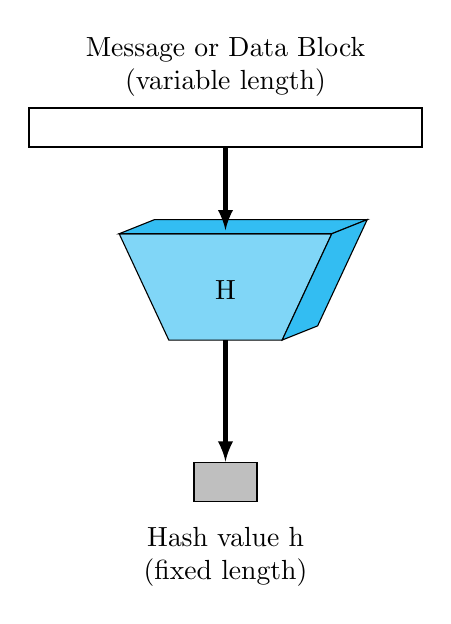
\begin{tikzpicture}[scale=0.9]
\node at (0,5) [draw, name=Message, rectangle, minimum width = 5cm, minimum height = 0.5cm, line width = 0.7pt]{};
\node [above=0.01cm of Message, align=center]{Message or Data Block\\(variable length)};
\draw[fill=cyan!50] (-0.8,2) -- (-1.5,3.5) -- (1.5,3.5) -- (0.8,2) -- cycle;
\draw[fill=cyan!80] (-1.5,3.5) -- (-1,3.7) -- (2,3.7) -- (1.5,3.5) -- cycle;
\draw[fill=cyan!80] (1.5,3.5) -- (2,3.7) -- (1.3,2.2) -- (0.8,2) -- cycle;
\node at (0,2.7){H};
\node at (0,0) [draw, name=Hash, rectangle, minimum width = 0.8cm, minimum height = 0.5cm, fill=gray!50]{};
\node [below=0.2cm of Hash, align=center]{Hash value h\\(fixed length)};
\draw [->, line width=1.5pt, >=latex] (Message) -- (0,3.55);
\draw [->, line width=1.5pt, >=latex] (0,2) -- (Hash);
\end{tikzpicture}
\caption{\label{fig:hachage}Hash function}
\end{figure}

This compression property is particularly useful in cryptography as it significantly reduces the amount of data to encrypt. In order to ensure the authenticity and integrity of a message, one needs only to encrypt the fixed length hash as opposed to the message in its entirety.

Cryptographic hash functions are fundamental components in a variety of information security applications, such as digital signature generation and verification, key derivation, and pseudorandom bit generation.

Currently, the most widely used cryptographic hash functions are \textsc{SHA-1} and \textsc{MD5}. They are both based on the Merkle-Damg\r{a}rd construction, which is defined in Chapter~\ref{chap:Merkle}. Despite the fact hash functions belonging to the \textsc{SHA-2} family (based on this construction and approved for use by the NIST in 2002) are still considered cryptographically secure, theoretical weaknesses have been found in their algorithms.

Some weaknesses appear to be inherent to the Merkle-Damg\r{a}rd construction and every algorithm based on it might suffer of these same vulnerabilities, particularly against differential cryptanalysis. In this case an attack on the Merkle-Damg\r{a}rd construction could be expanded to every algorithms based on it.

In order to provide resiliance against Merkle-Damg\r{a}rd construction weaknesses and future advances in hash function analysis, the NIST organised a public \textsc{SHA-3} Cryptographic Hash Algorithm Competition, in pursuance of a new family of cryptographic hash functions, which rely on fundamentally different design principles to the Merkle-Damg\r{a}rd construction.

The selected winner of the \textsc{SHA-3} competition is based on a construction called the \emph{sponge construction}, which is defined in Chapter~\ref{chap:Sponge}. Due to the particular properties of the sponge construction, as well as defining four new cryptographic hash functions, the standard approves two \emph{extendable output functions}. They are the first such functions the NIST\footnote{National Institute of Standards and Technology} has standardized.


%% CONVENTIONS NOTATIONS
\chapter{Conventions And Notations}
\section{Notations}
Let us introduce notations that will be kept all along the report:
\begin{itemize}
  \item $M$ refers to a bit string of arbitrary length, i.e. $M \in {\{0,1\}}^*$.
  \item $\vert M\vert$ denotes the bit-length of M.
  \item $A\vert \vert B$ denotes the concatenation of $A$ and $B$, where $A, B \in {\{0,1\}}^*$.
  \item $ M\vert \vert pad\lbrack r\rbrack (\vert M\vert )$ denotes the padding of a message M that is to be split into blocs of $r$ bits.
  \item $\vert M\vert_r$ denotes the number of blocs  of $r$ bits that M splits into once padded.
  \item $\lfloor M\rfloor_r$ denotes the truncation of a bitstring M to its first $r$ bits, $r\in \mathbb{N}$.
  \item For $a, b \in \mathbb{N}$, the notation  $\llbracket a,b \rrbracket$ is used to indicate the interval of all integers between a and b, including both. To indicate that one of the endpoints is to be excluded from the set, the corresponding square bracket is reversed.
  \item For a given set $\mathcal{E}$, $\# \mathcal{E}$ is the cardinal of $\mathcal{E}$.
\end{itemize}

\section{Padding Rules}\label{section:padding}

\begin{defn} \emph{Simple padding}, denoted by pad10∗, appends a single bit 1 followed by the minimum number of bits 0 such that the length of the result is a multiple of the block length.
Simple padding appends at least 1 bit and at most the number of bits in a block. 
\end{defn}

\begin{figure}[H]
  \centering
  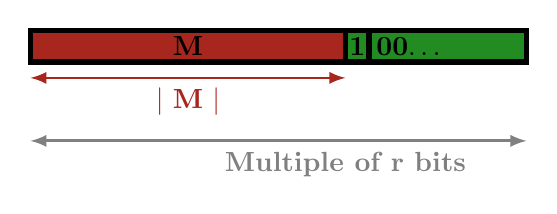
\begin{tikzpicture}[scale=1]
    
    \draw [name=green, fill=Mahogany, line width=2pt] (0,0) rectangle (4,0.4);
    \draw [fill=ForestGreen, line width=2pt] (4,0) rectangle (4.3,0.4);
    \draw [fill=ForestGreen, line width=2pt] (4.3,0) rectangle (6.3,0.4);

    \node [align=center] at (2,0.2){\textbf{M}};
    \node [align=center] at (4.15,0.2){\textbf{1}};
    \node [align=left]   at (4.8,0.2){\textbf{00}$\ldots$};
    
    \draw [<->, >=latex, line width=1pt, color=Mahogany] (0,-0.2) -- (4,-0.2);
    \draw [<->, >=latex, line width=1pt, color=Gray] (0,-1) -- (6.3,-1);

    \node [align=center, color=Mahogany] at (2,-0.5){$\vert$ \textbf{M} $\vert$};
    \node [align=center, color=Gray] at (4,-1.3){\textbf{Multiple of r\ bits}};
    
  \end{tikzpicture}
  \caption{\label{fig:SimplePadding}Simple padding.}
\end{figure}

Hashing functions based on the Merkle-Damg\r{a}rd construction, as defined in Section~\ref{sec:MerkleDamg}, use a similar padding rule to \emph{simple padding}. Simple padding is applied to obtain a message length of $r-64$ bits, after which the binary length of the original message, encoded as a 64-bit long integer, is appended to the padded message. The resulting length of the padded message $ M\vert \vert pad\lbrack r\rbrack (\vert M\vert )$ is $r\cdot \vert M\vert_{r}$ where $\vert M\vert_{r}$ is a positive integer (cf Figure~\ref{fig:MDPadding}).
\begin{figure}[H]
  \centering
  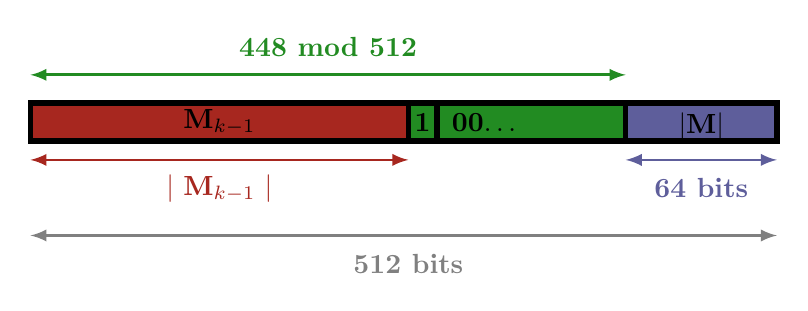
\begin{tikzpicture}[scale=1.2]
    
    \draw [name=green, fill=Mahogany, line width=2pt] (0,0) rectangle (4,0.4);
    \draw [fill=ForestGreen, line width=2pt] (4,0) rectangle (4.3,0.4);
    \draw [fill=ForestGreen, line width=2pt] (4.3,0) rectangle (6.3,0.4);
    \draw [fill=MidnightBlue!70, line width=2pt] (6.3,0) rectangle (7.9,0.4);

    \node [align=center] at (2,0.2){\textbf{M$_{k-1}$}};
    \node [align=center] at (4.15,0.2){\textbf{1}};
    \node [align=left]   at (4.8,0.2){\textbf{00}$\ldots$};
    \node [align=center] at (7.1,0.15){$\vert \textbf{M}\vert $};
    
    \draw [<->, >=latex, line width=1pt, color=Mahogany] (0,-0.2) -- (4,-0.2);
    \draw [<->, >=latex, line width=1pt, color=ForestGreen] (0,0.7) -- (6.3,0.7);
    \draw [<->, >=latex, line width=1pt, color=Gray] (0,-1) -- (7.9,-1);
    \draw [<->, >=latex, line width=1pt, color=MidnightBlue!70] (6.3,-0.2) -- (7.9,-0.2);

    \node [align=center, color=Mahogany] at (2,-0.5){$\vert$ \textbf{M$_{k-1}$} $\vert$};
    \node [align=center, color=ForestGreen] at (3.15,1){\textbf{448\ mod\ 512}};
    \node [align=center, color=Gray] at (4,-1.3){\textbf{512\ bits}};
    \node [align=center, color=MidnightBlue!70] at (7.1,-0.5){\textbf{64\ bits}};
    
  \end{tikzpicture}
  \caption{\label{fig:MDPadding}Merkle-Damg\r{a}rd padding.}
\end{figure}

For alternative hashing functions based on the sponge construction, as defined in Section~\ref{sec:Sponge}, we introduce an additional security constraint:
\begin{defn}A padding rule is \emph{sponge-compliant} if it never results in the empty string and if it satisfies following criterion:
$$\forall n \ge 0\mbox{, } \forall M, M' ∈ \mathbb Z_2^* \mbox{: } M \ne M′ \Rightarrow \mbox{ }M\vert \vert pad \lbrack r\rbrack(\vert M\vert ) \ne M'\vert \vert pad\lbrack r \rbrack (\vert M'\vert )\vert \vert 0^{nr}$$
\end{defn}

\emph{Simple padding} the simplest padding rule that is sponge-compliant. The simplest padding rule that allows securely using the same f with different rates is the following:
\begin{defn} \emph{Multi-rate} padding, denoted by pad10∗1, appends a single bit 1 followed by the minimum number of bits 0 followed by a single bit 1 such that the length of the result is a multiple of the block length.
Clearly, this padding rule is sponge-compliant as well as it is injective and cannot result in an empty string or a string with all-zero last block. Multi-rate padding appends at least 2 bits and at most the number of bits in a block plus one.
\end{defn}


\begin{figure}[H]
  \centering
  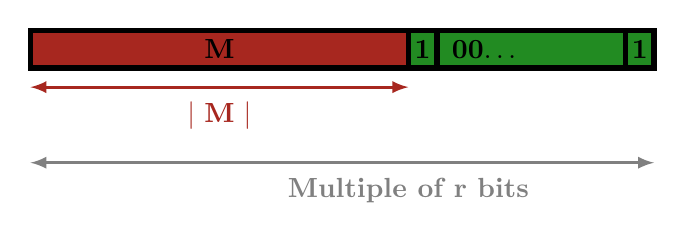
\begin{tikzpicture}[scale=1.2]
    
    \draw [name=green, fill=Mahogany, line width=2pt] (0,0) rectangle (4,0.4);
    \draw [fill=ForestGreen, line width=2pt] (4,0) rectangle (4.3,0.4);
    \draw [fill=ForestGreen, line width=2pt] (4.3,0) rectangle (6.3,0.4);
    \draw [fill=ForestGreen, line width=2pt] (6.3,0) rectangle (6.6,0.4);

    \node [align=center] at (2,0.2){\textbf{M}};
    \node [align=center] at (4.15,0.2){\textbf{1}};
    \node [align=left]   at (4.8,0.2){\textbf{00}$\ldots$};
    \node [align=center] at (6.45,0.2){\textbf{1}};
    
    \draw [<->, >=latex, line width=1pt, color=Mahogany] (0,-0.2) -- (4,-0.2);
    \draw [<->, >=latex, line width=1pt, color=Gray] (0,-1) -- (6.6,-1);

    \node [align=center, color=Mahogany] at (2,-0.5){$\vert$ \textbf{M} $\vert$};
    \node [align=center, color=Gray] at (4,-1.3){\textbf{Multiple of r\ bits}};
    
  \end{tikzpicture}
  \caption{\label{fig:MultiPadding}Multi-rate padding.}
\end{figure}



%% PART 1
\chapter{Hashing Algorithms Based On The Merkle-Damg\r{a}rd  Construction}\label{chap:Merkle}

Nowadays, one-way hash functions are used in many cryptographic applications.\\
They are used for authentification, integrity checking, encryption and digital signatures (with public-key algorithms) and many security protocols. That's why, in order to guarantee their cryptographic robustness, they need to comply with various rules.

\section{Overview}

%Mathematical Purpose:
For many reasons, hash functions need to be one-way functions.
Ideally, each digest output by a hash function would match with a single input message. This would guarantee the source message is the one we really expect, and that no different message could have been sent resulting in the same digest.

However in practice, such a property is not feasible, as hashing functions also guarantee a compression property, mapping an infinite starting set to a finite codomain.
Hash functions must therefore attempt, as far as possible, to avoid what are called collisions (two messages resulting in the same hash).

Moreover it is important that one cannot retrieve the original message, using only its hash.
If it were possible, the hash function would be useless, a malicious individual could compute a message resulting in a given hash, enabling him to send a different message than the one initially intended but using the same digest, and therefore the hash function would no longer guarantee a message's authenticity. For these reasons one-way hash functions need to respect various properties.

%Merkle-Damgard
To guarantee all these properties, it is often safest to ensure hashing functions follow established patterns to be fully efficient. Here, we will study hash functions based on the Merkle-Damg\r{a}rd construction. 


\section{Cryptographic Requirements Of A Hash Function}~\label{sec:requirements}

One major requirement when building a hash functions is that it must be efficient, and therefore easy to compute. 
Other properties may also be required for cryptographic purposes.

\begin{defn}A collision between two different messages is a situation that occurs when two different messages $x \ne x'$ have the same hash value $H(x) = H(x')$.
\end{defn}
\begin{rem}
In so far as the input message of a hashing function can be of any length (in particular greater than the length of the output diggest), collisions are unavoidable.
\end{rem}
\begin{defn}
If y is such that $y = H(x)$, then x is a \emph{pre-image} for y (y being the \emph{hash} or \emph{digest}  of x).
\end{defn}

\begin{defn}~\label{def:sec_prop}
Hereafter are the three main properties a cryptographic hash function must fulfill:
\begin{itemize}
\item \textbf{Pre-image resistance}:  given $y$, it is hard to find a pre-image $x \in f^{-1}(H)$ such that $y = H(x)$.
\item \textbf{Second pre-image resistance}: given $x$, it is hard to find $x' \ne x$ such that $H(x) = H(x')$.
\item \textbf{Collision resistance}: it is hard to find two different messages $x' \ne x$ that have the same hash $H(x) = H(x')$.
\end{itemize}
\end{defn}

\begin{prop}Resistance to collisions implies second pre-image resistance which in turn implies pre-image resistance.
\end{prop}


\section{The Merkle-Damg\r{a}rd Construction}\label{sec:MerkleDamg}

The well known Merkle-Damg\r{a}rd construction describes how to construct a hash function based on a general compression function in an iterative structure. 

\begin{defn}A \emph{compression function} is a fixed input-size function which has an output length smaller than its input length: 
$$h:{\{0,1\}}^b ×{\{0,1\}}^n \rightarrow {\{0,1\}}^n$$
as depicted in figure~\ref{fig:compression}.
\end{defn}

\begin{figure}[H]
\centering
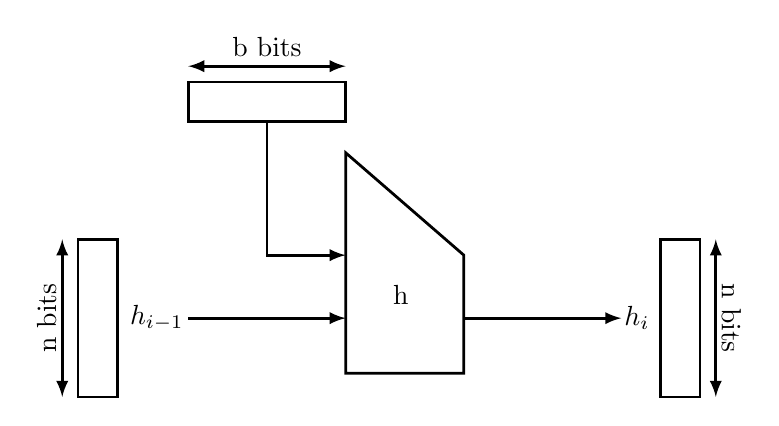
\begin{tikzpicture}

\draw[line width=1pt, name=h] (0,0) -- (0,2.8) -- (1.5,1.5) -- (1.5,0) -- cycle;
\node at(0.7,1){h};

\draw[line width=1pt] (-2,3.2) -- (0,3.2) -- (0,3.7) -- (-2,3.7) -- cycle;
\draw[<->, line width=1pt, >=latex] (-2,3.9) -- (0,3.9);
\node at (-1,4.15){b bits};
\draw[->, line width=1pt, >=latex] (-1,3.2) -- (-1,1.5) -- (0,1.5);


\draw[line width=1pt] (-3.4,-0.3) -- (-2.9,-0.3) -- (-2.9,1.7) -- (-3.4,1.7) -- cycle;
\node at (-2.4,0.7){$h_{i-1}$};
\draw[<->, line width=1pt, >=latex] (-3.6,-0.3) -- (-3.6,1.7);
\node[rotate=90] at (-3.8, 0.7){n bits};
\draw[->, line width=1pt, >=latex] (-2,0.7) -- (0,0.7);

\draw[line width=1pt] (4,-0.3) -- (4.5,-0.3) -- (4.5,1.7) -- (4,1.7) -- cycle;
\node at (3.7,0.7){$h_{i}$};
\draw[->, line width=1pt, >=latex] (1.5,0.7) -- (3.5,0.7);
\node[rotate=270] at (4.9, 0.7){n bits};
\draw[<->, line width=1pt, >=latex] (4.7,-0.3) -- (4.7,1.7);

\end{tikzpicture}
\caption{\label{fig:compression}Compression function.}
\end{figure}


Input values for the Merkle-Damg\r{a}rd construction are an n-bit IV (\emph{Initial Value}) and the arbitrary length input message. 
The IV is a fixed public value.

First the message $M$ is padded so that the entire padded message length be a multiple of the message block length b. The padded message is then separated into blocs of size exactly $b$ bits: $M_0,\ldots,M_{k-1}$.

The compression function h is then iterated according to the model depicted in figure~\ref{fig:constructionMD}.

\begin{figure}[ht]
\centering
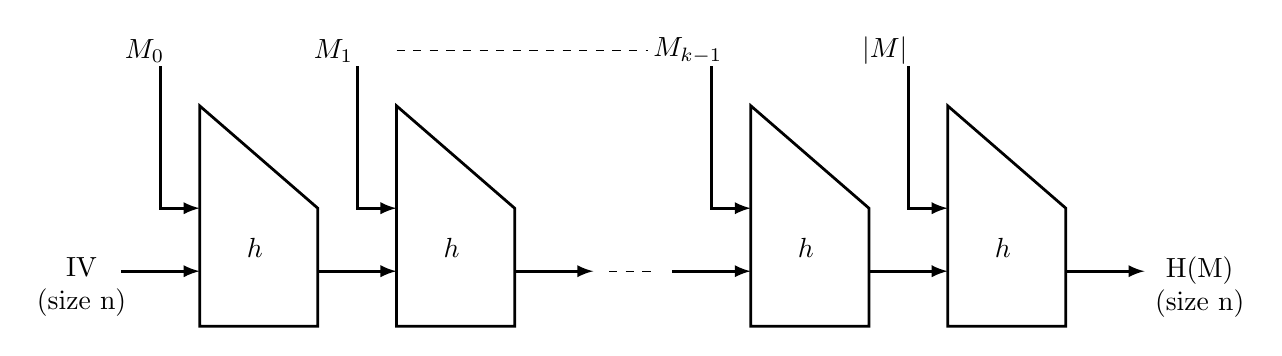
\begin{tikzpicture}

\node at (-0.7,3.5){$M_{0}$};
\draw[->, >=latex, line width=1pt] (-0.5,3.3) -- (-0.5,1.5) -- (0,1.5);
\node[align=center] at (-1.5,0.5){IV\\(size n)};
\draw[->, >=latex, line width=1pt] (-1,0.7) -- (0,0.7);
\draw[line width=1pt] (0,0) -- (0,2.8) -- (1.5,1.5) -- (1.5,0) -- cycle;
\node at(0.7,1){$h$};

\node at (1.7,3.5){$M_{1}$};
\draw[->, >=latex, line width=1pt] (2,3.3) -- (2,1.5) -- (2.5,1.5);
\draw[->, >=latex, line width=1pt] (1.5,0.7) -- (2.5,0.7);
\draw[line width=1pt] (2.5,0) -- (2.5,2.8) -- (4,1.5) -- (4,0) -- cycle;
\node at(3.2,1){$h$};
\draw[->, >=latex, line width=1pt] (4,0.7) -- (5,0.7);

\draw[dashed] (5.2,0.7) -- (5.8,0.7);
\draw[dashed] (2.5,3.5) -- (5.7,3.5);

\node at (6.2,3.5){$M_{k-1}$};
\draw[->, >=latex, line width=1pt] (6.5,3.3) -- (6.5,1.5) -- (7,1.5);
\draw[->, >=latex, line width=1pt] (6,0.7) -- (7,0.7);
\draw[line width=1pt] (7,0) -- (7,2.8) -- (8.5,1.5) -- (8.5,0) -- cycle;
\node at(7.7,1){$h$};

\node at (8.7,3.5){$|M|$};
\draw[->, >=latex, line width=1pt] (9,3.3) -- (9,1.5) -- (9.5,1.5);
\draw[->, >=latex, line width=1pt] (8.5,0.7) -- (9.5,0.7);
\draw[line width=1pt] (9.5,0) -- (9.5,2.8) -- (11,1.5) -- (11,0) -- cycle;
\node at(10.2,1){$h$};
\draw[->, >=latex, line width=1pt] (11,0.7) -- (12,0.7);
\node[align=center] at (12.7,0.5){H(M)\\(size n)};

\end{tikzpicture}
\caption{\label{fig:constructionMD}Merkle-Damg\r{a}rd construction.}
\end{figure}

A theorem demonstrated independently by Ralph Merkle and Ivan Damg\r{a}rd defines the theoretical properties of such a construction:
\begin{thm}
If the compression function $h$ is resistant to collision functions, then the resulting hash function $H$ is also.
\end{thm}


\begin{proof}
  We shall prove the theorem by contradiction:

  Let us assume that $H$ is not resistant to collisions, which means we can easily find $M$ and $M'$, such that $M \ne M'$ and $H(M)=H(M')$.
  Let us define $k$ and $l$ such that $k=\vert M\vert_b$ with $k \ge 1$ and $l=\vert M'\vert_b$ with $l \ge k$.
  We also define $y_0 = h^{k-1}(M)$ and $y_0' = h^{l-1}(M')$.\\
  Three cases may occur:
\begin{itemize}
\item Either $M_0,\ldots,M_{k-2}=M_0',\ldots,M_{k-2}'= u $. In which case $h(u \vert \vert M_{k-1})=h(u \vert \vert M_{k-1}',\ldots,M_{l-1}')$ we have found a collision for $h$.
\item Either $y_0 \ne y_0'$ and then since $h(y_0)=h(y_0')=H(M)=H(M')$ we have found a collision for $h$.
\item Either $y_0 = y_0'$ and $M_0,\ldots,M_{k-2} \ne M_0',\ldots,M_{k-2}'$. In which case we repeat the procedure with $y_i = h^{k-1-i}(M)$ and $y_i' = h^{l-1-i}(M')$ until $y_i \ne y_i'$.
\end{itemize}
\end{proof}


\paragraph{}

Consequently Merkle-Damg\r{a}rd is the most widespread construction used in calculating hashes.

Based on this construction, MD4 and MD5 formed an inspiration for other hash function designs that have followed over the years. They are all based on the Merkle-Damg\r{a}rd construction and have similar basic designs for their compression functions. The MD and SHA family of hash functions include (among others): MD4, MD5, SHA-0, SHA-1, the SHA2 family, RIPEMD \ldots





\section{MD5}

MD5, designed by Ronald Rivest in 1991, is a widely used cryptographic hash function. Based on the Merkle-Damg\r{a}rd construction, this one-way function produces a 128-bit digest, usually presented in text format as a 32 digit hexadecimal number.

\subsection{MD5 Overview}
\cite{Att}
Let us now explain how the MD5 algorithm operates on a given input M, where M is an arbitrary length bit string.
\begin{enumerate}
\item \emph{Padding}: The original message is padded so that the resulting length of $ M\vert \vert pad\lbrack 512\rbrack (\vert M\vert )$ is $512\cdot \vert M\vert_{512}$ where $\vert M\vert_{512}$ is a positive integer.

\item \emph{Partitioning}: The padded message $P= M\vert \vert pad\lbrack 512\rbrack (\vert M\vert )$ is split into $N=\vert M\vert_{512}$ consecutive blocs that are each 512 bits long:\\ $M_0, M_1,\ldots, M_{N−1}$.

\item \emph{Processing}: In order to hash a message that is made up of $N$ blocks, MD5 iterates through $N + 1$ states $IHV_i$, for $0 \le i \le N$, called \emph{intermediate hash values}. Each intermediate hash value $IHV_i$ is a tuple of four 32-bit words $(a_i, b_i, c_i, d_i)$. For $i = 0$, the tuple has a fixed public value, called \emph{initial value} $(IV)$:
$$(a_0,b_0,c_0,d_0) = (67452301_{16},efcdab89_{16},98badcfe_{16},10325476_{16}).$$

For $i = 1,2,\ldots,N$ the intermediate hash value $IHV_i$ is computed using MD5's compression function. This step is detailed in~\ref{sec:compressionMD5}:
$$IHV_i = \textsc{MD5Compress}(IHV_{i−1},M_{i−1}).$$

\item  \emph{Output}: The resulting hash value, $IHV_N$, is expressed as the concatenation of the hexadecimal byte strings of the four words $a_N , b_N , c_N , d_N$, converted back from their little-endian representation. An example of  $IHV_N$ could be:
 $$0123456789abcdeffedcba9876543210_{16}$$

\end{enumerate}
\subsection{MD5 Compression Function}\label{sec:compressionMD5}
The inputs of \textsc{MD5Compress} ($IVH_i$,$M_i$), producing the $i+1{th}$ intermediate hash value, are an intermediate hash value $IHV_{i}=(a,b,c,d)$ and a 512-bit block of the original message. The compression function iterates through 64 \emph{steps}, split into four consecutive \emph{rounds} of 16 steps each. Each step $t$ uses modular additions, a left rotation, a non-linear function $f_t$, an \emph{additional constant} $AC_t$ and a  \emph{rotation Constant} $RC_t$.

These constants are defined as follows:
\begin{equation}
AC_t = \lfloor 2^{32} \vert \sin(t+1)\vert \rfloor \mbox{, }  0\le t\le 64
\end{equation}
\begin{equation}
(RC_t, RC_{t+1}, RC_{t+2}, RC_{t+3})
\begin{cases}
(7, 12, 17, 22) & \mbox{ for } t = 0,4,8,12; \\
(5, 9, 14, 20) & \mbox{ for } t = 16, 20, 24, 28;\\
(4, 11, 16, 23) & \mbox{ for } t = 32, 36, 40, 44; \\
(6, 10, 15, 21) & \mbox{ for } t = 48,52,56,60; \\
\end{cases}
\end{equation}

The non-linear function $f_t$ depends on the round:

\begin{equation}
f_t(X,Y,Z)
\begin{cases}
F(X, Y, Z) = (X \wedge Y) \oplus (\overline{X} \wedge Z) & \mbox{ if } 0 \le t < 16; \\
G(X, Y, Z) = (Z \wedge X) \oplus (\overline{Z} \wedge Y) & \mbox{ if } 16 \le t < 32; \\
H(X, Y, Z) = X \oplus Y \oplus Z & \mbox{ if } 32 \le t < 48; \\
I(X, Y, Z) = Y \oplus (X \vee \overline{Z}) & \mbox{ if } 48 \le t < 64; \\
\end{cases}
\end{equation}

The 512-bit input message block $M_i$, of the original message, is divided into sixteen 32-bit long words $m_0,m_1,\ldots,m_{15}$ (using \emph{little endian} byte ordering). These words are then extended into 64 32-bit words $W_t$ for $0 \le t < 64$:
\begin{equation}
W_t =
\begin{cases}
m_t & \mbox{ for } 0 \le t < 16; \\
m_{(1+5t)\mbox{ mod }16} & \mbox{ for } 16 \le t < 32; \\
m_{(5+3t)\mbox{ mod }16} & \mbox{ for } 32 \le t < 48; \\
m_{(7t)\mbox{ mod }16} & \mbox{ for } 48 \le t < 64; \\
\end{cases}
\end{equation}

\begin{figure}[!ht]
  \centering
  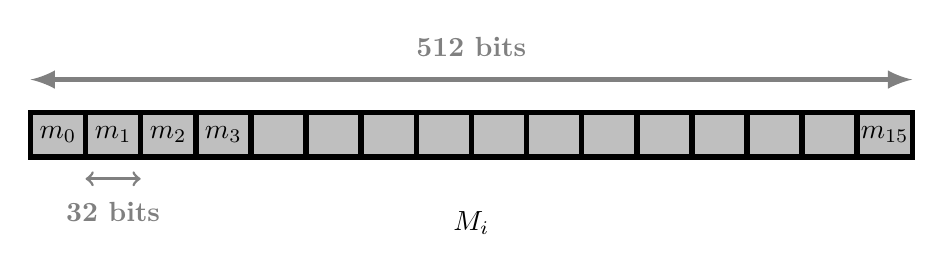
\begin{tikzpicture}[scale=1.4]

    \draw [fill=Gray!50, line width=2pt] (0,0) rectangle (0.5,0.4) node[pos=.5]{\textbf{$m_{0}$}};
    \draw [fill=Gray!50, line width=2pt] (0.5,0) rectangle (1,0.4) node[pos=.5]{\textbf{$m_{1}$}};
    \draw [fill=Gray!50, line width=2pt] (1,0) rectangle (1.5,0.4) node[pos=.5]{\textbf{$m_{2}$}};
    \draw [fill=Gray!50, line width=2pt] (1.5,0) rectangle (2,0.4) node[pos=.5]{\textbf{$m_{3}$}};
    \draw [fill=Gray!50, line width=2pt] (2,0) rectangle (2.5,0.4);
    \draw [fill=Gray!50, line width=2pt] (2.5,0) rectangle (3,0.4);
    \draw [fill=Gray!50, line width=2pt] (3,0) rectangle (3.5,0.4);
    \draw [fill=Gray!50, line width=2pt] (3.5,0) rectangle (4,0.4);
    \draw [fill=Gray!50, line width=2pt] (4,0) rectangle (4.5,0.4);
    \draw [fill=Gray!50, line width=2pt] (4.5,0) rectangle (5,0.4);
    \draw [fill=Gray!50, line width=2pt] (5,0) rectangle (5.5,0.4);
    \draw [fill=Gray!50, line width=2pt] (5.5,0) rectangle (6,0.4);
    \draw [fill=Gray!50, line width=2pt] (6,0) rectangle (6.5,0.4);
    \draw [fill=Gray!50, line width=2pt] (6.5,0) rectangle (7,0.4);
    \draw [fill=Gray!50, line width=2pt] (7,0) rectangle (7.5,0.4);
    \draw [fill=Gray!50, line width=2pt] (7.5,0) rectangle (8,0.4) node[pos=.5]{\textbf{$m_{15}$}};

    \draw [<->, >=latex, line width=2pt, color=Gray] (0,0.7) -- (8,0.7);
    \draw [<->, line width=1pt, color=Gray] (0.5,-0.2) -- (1,-0.2);

    \node [align=center, color=Gray] at (4,1){\textbf{512 bits}};
    \node [align=center, color=Gray] at (0.75,-0.5){\textbf{32 bits}};
    \node [align=center] at (4,-0.6){\textbf{$M_i$}};
    
  \end{tikzpicture}
  \caption{\label{fig:B}$M_i$ is divided into sixteen 32-bit words.}
\end{figure}

For each step t, the compression function uses a working state, consisting of four 32-bit words $Q_t, Q_{t-1}, Q_{t-2}$ and $Q_{t-3}$ and computes a new word of the working state $Q_{t+1}$. The initial value of the working state is  $(Q_0, Q_{-1}, Q_{-2},Q_{-3}) = (b,c,d,a)$.

For $t=0,1,\ldots,63$, the subsequent working state $Q_{t+1}$ is computed as follows:
\begin{equation}
\begin{aligned}
  &F_t = f_t(Q_t, Q_{t-1}, Q_{t-2}); \\
  &T_t = F_t + Q_{t-3} + AC_t + W_t; \\
  &R_t = RL(T_t,RC_t); \\
  &Q{t_+1} = Q_t +R_t; \\
\end{aligned}
\end{equation}

Once all the steps have been computed, the resulting state words are added to the input intermediate hash values, and returned as output:
\begin{equation}
MD5Compress(IHV_{i}, M_i) = (a + Q_{61}, b + Q_{64}, c + Q_{63}, d + Q_{62}).
\end{equation}

\subsection{MD5 Algorithm}~\label{section:md5}
The pseudo-code for the MD5 algorithm is presented in Algorithm~\ref{algo:md5}.
\begin{algorithm}[H]
\caption{MD5(x)}
\label{algo:md5}
\begin{algorithmic}[1]
\State{\textbf{external procedures} MD5-\textsc{pad}}
\State{let us call $RC\lbrack 64\rbrack$ the array of rotation constants.}
\State{let us call $AC\lbrack 64\rbrack$ the array of additional constants.}
\State{$RC\lbrack 0{\ldots}15\rbrack \gets \{7, 12, 17, 22,  7, 12, 17, 22,  7, 12, 17, 22,  7, 12, 17, 22\}$}
\State{$RC\lbrack 16{\ldots}31\rbrack \gets \{5,  9, 14, 20,  5,  9, 14, 20,  5,  9, 14, 20,  5,  9, 14, 20\}$}
\State{$RC\lbrack 32{\ldots}47\rbrack \gets \{4, 11, 16, 23,  4, 11, 16, 23,  4, 11, 16, 23,  4, 11, 16, 23\}$}
\State{$RC\lbrack 48{\ldots}63\rbrack \gets \{6, 10, 15, 21,  6, 10, 15, 21,  6, 10, 15, 21,  6, 10, 15, 21\}$}

\For{$i \gets 0$ to $63$ }
\State{$AC\lbrack i\rbrack \gets \lfloor 2^{32} \vert \sin(t+1)\vert \rfloor$}
\EndFor{}

\Comment{Initialise variables}
\State{$a_0 \gets \mbox{0x67452301}$}
\State{$b_0 \gets \mbox{0xefcdab89}$}
\State{$c_0 \gets \mbox{0x98badcfe}$}
\State{$d_0 \gets \mbox{0x10325476}$}

\State{$M_1 \vert \vert M_2 \vert \vert \ldots \vert \vert M_N \gets$ MD5-\textsc{pad} (x), where each  $M_i$ is a 512-bit block.}

\Comment{Loop through all $N$ message blocs to hash.}
\For{$i \gets 1$ to $N$ }
\State{let us call $W\lbrack 16\rbrack$ the array of 32-bit words in $M_i$. }
\State{$M_i = W\lbrack 0\rbrack \vert \vert W\lbrack 1\rbrack \vert \vert \ldots vert \vert W\lbrack 15\rbrack$.}

\Comment{Initial values}
\State{$a \gets a_0$}
\State{$b \gets b_0$}
\State{$c \gets c_0$}
\State{$d \gets d_0$}

\Comment{Iterate through the 64 steps of the compression function}
\For{$t \gets 0$ to $63$ }
\If{$0\le i \le 15$}
\Comment{$f_t$ is F and $W_t$ is $m_t$}
\State{$f \gets (b \wedge c) \oplus (\overline{b} \wedge d)$}
\State{$g \gets t$}

\ElsIf{$16\le i \le 31$}
\Comment{$f_t$ is G and $W_t$ is $m_{1+5t}$}
\State{$f \gets (d \wedge b) \oplus (\overline{d} \wedge c)$}
\State{$g \gets (5*t+1) \mod{16}$}

\ElsIf{$32\le i \le 47$}
\Comment{$f_t$ is H and $W_t$ is $m_{5+3t}$}
\State{$f \gets b \oplus c \oplus d$}
\State{$g \gets (3*t+5) \mod{16}$}

\ElsIf{$48\le i \le 63$}
\Comment{$f_t$ is I and $W_t$ is $m_{7t}$}
\State{$f \gets c \oplus (b \vee \overline{d})$}
\State{$g \gets (7*t) \mod{16}$}
\EndIf{}

\State{$temp \gets d$}
\State{$d \gets c$}
\State{$c \gets b$}
\State{$b \gets ((a + f + AC\lbrack t \rbrack + W\lbrack g \rbrack)) +b $}
\State{$a \gets temp$}
\EndFor{}

\Comment{Once all the steps have been computed, the resulting state words are added to the input intermediate hash values}
\State{$a_0 \gets a_0 + a$}
\State{$b_0 \gets b_0 + b$}
\State{$c_0 \gets c_0 + c$}
\State{$d_0 \gets d_0 + d$}

\EndFor{}

\Return{$digest \gets a_0 \vert \vert b_0 \vert \vert c_0 \vert \vert d_0 \vert \vert H_4$}

\Comment{Return output as little endian}
\end{algorithmic}
\end{algorithm}

\section{SHA-1}
\textsc{SHA-1} was published in 1995 by the NIST as a standard, it is another hash algorithm, based on the Merkle-Damg\r{a}rd construction, which is widely implemented, though is deprecated as it is also considered cryptographically broken (see Chapter~\ref{chap:security}). It is still used due to legacy systems that do not have the support for SHA-2 or SHA-3.

SHA-1 pads the input message $M$, then splits it into $n$ blocs $M_1, M_2, {\ldots} ,M_n$ that are each $b=512$ bits long.
We shall focus here on the operations performed on a bloc $M_i$.
The compression function takes as an input a $512$-bit long message block and produces a $160$ bit long digest.

\subsection{Defining SHA-1 Constants And Functions}

\begin{itemize}
\item The \textsc{SHA-1} padding function pads the original message into $N=\vert M\vert_{512}$ consecutive blocs that are each 512 bits long: $M_0, M_1,{\ldots}, M_{N−1}$.

$$ M\vert \vert pad\lbrack 512\rbrack (\vert M\vert ) = M_0 \vert \vert M_1 \vert \vert \ldots \vert \vert M_{N-1}$$
\item A cyclic shift of x of k positions to the left is defined as:
$$RL(x,k)=(x<<k)\lor (x>>32-k)$$

\item Functions $F_0, {\ldots}, F_{79}$ are defined as follows:
\begin{equation}
F_t(B,C,D) =
\begin{cases}
(B \wedge C)  \vee (\overline{B} \wedge D) & \mbox{ for }0 \le t \le 19 \\
B \oplus C \oplus D & \mbox{ for } 20 \le t \le 39 \\
(B \wedge C)  \vee (B \wedge D)  \vee (C \wedge D) & \mbox{ for }40\le t\le 59 \\ 
B \oplus C \oplus D & \mbox{ for }60\le t\le 79 
\end{cases}
\end{equation}
Each function $F_t$ takes as inputs three 32-bit words and outputs one 32-bit word.

\item Constants $K_0, K_1, {\ldots}, K_{79}$, are defined as follows:
\begin{equation}
K_t =
\begin{cases}
\mbox{0x5a827999} & \mbox{ for }0 \le t \le 19 \\
\mbox{0x6ed9eba1} & \mbox{ for }20 \le t\le 39 \\ 
\mbox{0x8f1bbcdc} & \mbox{ for }40\le t\le 59 \\ 
\mbox{0xca62c1d6} & \mbox{ for }60\le t\le 79 
\end{cases}
\end{equation}
 \item The compression function iterates through 80 rounds for each input message bloc. Each one of these rounds performs the operations depicted in Figure~\ref{fig:SHA-1}
\end{itemize}

\begin{figure}[!ht]
        \centering
        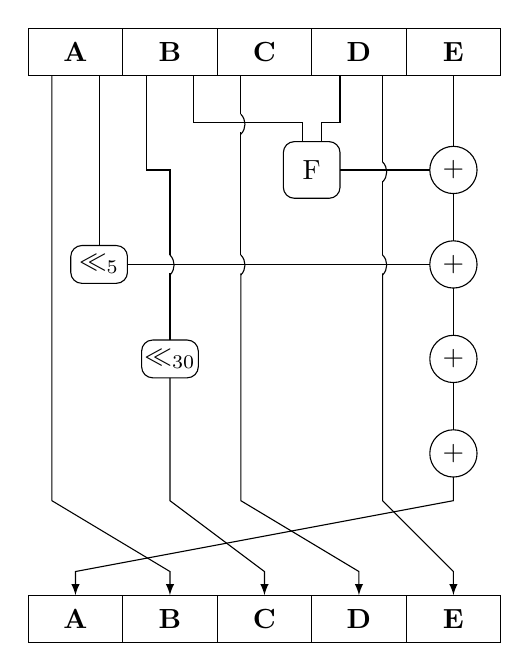
\begin{tikzpicture}[scale=1.2]
        %Box Messages
        \draw  (0,0) rectangle (1,0.5); \node [align=center] at (0.5,0.25){\textbf{A}};
        \draw  (1,0) rectangle (2,0.5); \node [align=center] at (1.5,0.25){\textbf{B}};
        \draw  (2,0) rectangle (3,0.5); \node [align=center] at (2.5,0.25){\textbf{C}};
        \draw  (3,0) rectangle (4,0.5); \node [align=center] at (3.5,0.25){\textbf{D}};
        \draw  (4,0) rectangle (5,0.5); \node [align=center] at (4.5,0.25){\textbf{E}};
        \draw  (0,6) rectangle (1,6.5); \node [align=center] at (0.5,6.25){\textbf{A}};
        \draw  (1,6) rectangle (2,6.5); \node [align=center] at (1.5,6.25){\textbf{B}};
        \draw  (2,6) rectangle (3,6.5); \node [align=center] at (2.5,6.25){\textbf{C}};
        \draw  (3,6) rectangle (4,6.5); \node [align=center] at (3.5,6.25){\textbf{D}};
        \draw  (4,6) rectangle (5,6.5); \node [align=center] at (4.5,6.25){\textbf{E}};
        %Cercles
        \draw  (4.5,5) circle (0.25); \node [align=center] at (4.5,5){+};
        \draw  (4.5,4) circle (0.25); \node [align=center] at (4.5,4){+};
        \draw  (4.5,3) circle (0.25); \node [align=center] at (4.5,3){+};
        \draw  (4.5,2) circle (0.25); \node [align=center] at (4.5,2){+};
        %Boxs + Textes
        \draw  [rounded corners] (2.7,4.7) rectangle (3.3,5.3); \node [align=center] at (3,5){F};
        \draw  [rounded corners] (0.45,3.8) rectangle (1.05,4.2); \node [align=center] at (0.75,4){$\ll_5$};
        \draw  [rounded corners] (1.2,2.8) rectangle (1.8,3.2); \node [align=center] at (1.5,3){$\ll_{30}$};
        %Traits et Fleches
        \draw [->, >=latex] (0.25,6) -- (0.25,1.5) -- (1.5,0.75) -- (1.5,0.5);
        \draw [-] (4.5,6) -- (4.5,5.25);\draw [-] (4.5,4.75) -- (4.5,4.25);\draw [-] (4.5,3.75) -- (4.5,3.25);\draw [-] (4.5,2.75) -- (4.5,2.25);\draw [->, >=latex] (4.5,1.75) -- (4.5,1.5) -- (0.5,0.75) -- (0.5,0.5);
        \draw [-] (1.25,6) -- (1.25,5) -- (1.5,5) -- (1.5,4.1);\draw [-] (1.5,3.905) -- (1.5,3.2);\draw [->, >=latex] (1.5,2.8) -- (1.5,1.5) -- (2.5,0.75) -- (2.5,0.5);
        \draw [-] (2.25,6) -- (2.25,5.59);\draw [-] (2.25,5.4) -- (2.25,4.1);\draw [->, >=latex] (2.25,3.905) -- (2.25,1.5) -- (3.5,0.75) -- (3.5,0.5);
        \draw [-] (3.75,6) -- (3.75,5.085);\draw [-] (3.75,4.88) -- (3.75,4.1);\draw [->, >=latex] (3.75,3.905) -- (3.75,1.5) -- (4.5,0.75) -- (4.5,0.5);
        \draw [-] (0.75,6) -- (0.75,4.2);\draw [-] (1.05,4) -- (4.25,4);
        \draw [-] (1.75,6) -- (1.75,5.5) -- (2.9,5.5) -- (2.9,5.3);\draw [-] (3.3,6) -- (3.3,5.5) -- (3.1,5.5) -- (3.1,5.3);\draw [-] (3.3,5) -- (4.25,5);
        %Arcs de cercle
        \draw (2.25,5.59) arc(45:-45:0.15cm);\draw (2.25,4.1) arc(45:-45:0.15cm);\draw (1.5,4.1) arc(45:-45:0.15cm);\draw (3.75,4.1) arc(45:-45:0.15cm);\draw (3.75,5.085) arc(45:-45:0.15cm);

        \end{tikzpicture}
        \caption{\label{fig:SHA-1}The $i^{th}$ round in SHA-1 $(0\le i \le 79)$.}
\end{figure}

\clearpage

\subsection{SHA-1 Algorithm}\label{section:sha1}
The pseudo-code for the SHA-1 algorithm is presented in Algorithm~\ref{algo:sha1}.

\begin{algorithm}[H]
\caption{SHA-1(x)}
\label{algo:sha1}
\begin{algorithmic}[1]
\State{\textbf{external procedures} SHA-1-\textsc{pad}}
\State{\textbf{global variables} $K_0, {\ldots},K_{79}$}
\State{$y \gets$ SHA-1-\textsc{pad} (x)}
\State{Define $y = M_1 \vert \vert M_2 \vert \vert \ldots \vert \vert M_N$, where each  $M_i$ is a 512-bit block.}
\State{$H_0 \gets \mbox{0x67452301}$}
\State{$H_1 \gets \mbox{0xefcdab89}$}
\State{$H_2 \gets \mbox{0x98badcfe}$}
\State{$H_3 \gets \mbox{0x10325476}$}
\State{$H_4 \gets \mbox{0xc3d2e1f0}$}
\For{$i \gets 1$ to $N$ }
\State{Define $M_i = W_0 \vert \vert W_1 \vert \vert \ldots \vert \vert W_{15}$, where each $W_j$ is a 32-bit word.}

\For{$t \gets 16$ to $79$ }
\State{$W_t \gets RL(W_{t-3}\oplus W_{t-8}\oplus W_{t-14}\oplus W_{t-16}, 1)$}
\EndFor{} 

\State{$A \gets H_0$}
\State{$B \gets H_1$}
\State{$C \gets H_2$}
\State{$D \gets H_3$}
\State{$E \gets H_4$}

\For{$t \gets 0$ to $79$ }
\State{$tmp \gets RL(A, 5) + f_t(B,C,D) + E + W_t + K_t$}
\State{$E \gets D$}
\State{$D \gets C$}
\State{$C \gets RL(B,30)$}
\State{$B \gets A$}
\State{$A \gets tmp$}
\EndFor{}

\State{$H_0 \gets H_0 + A$}
\State{$H_1 \gets H_1 + B$}
\State{$H_2 \gets H_2 + C$}
\State{$H_3 \gets H_3 + D$}
\State{$H_4 \gets H_4 + E$}
\EndFor{}

\Return{$H_0 \vert \vert H_1 \vert \vert H_2 \vert \vert H_3 \vert \vert H_4$}
\end{algorithmic}
\end{algorithm}

\clearpage


%% PART 2
\chapter{Cryptographic Security And Known Attacks}
%\chapter{Near-Collision Attack}
 %INTRODUCTION  --> TODO Birthday Attack + General Attack
%TODO 
The main property a hash function must comply to is resitance to collisions (see Section~\ref{sec:requirements}). Therefore, a hashing algorithm is considered to be \emph{broken} if there exists a known attack that enables one to find collisions for the hash function with a time complexity less than a brute force attack.

All the attacks detailed below focus on finding \emph{collisions}. Since resistance to collision attacks implies resistance to pre-image and second pre-image attacks this is the strongest of the cryptographic requirements stated in Section~\ref{sec:requirements}.

We shall hereafter detail what a brute force (also known as Yuval's) attack is, and it's complexity, before exhibiting a few more specific attacks, and their consequences on public confidence in the robustness of algorithms based on the Merkle-Damg\r{a}rd construction.

\section{Brute Force Attack (Yuval's Attack)}
A brute force attack is a trial and error method. A large number of random consecutive guesses are made and the attack is successful if a guess leads to the desired output.

It can be compared to trying many random combinations on a padlock, in which case the attack is successful if the attacker is lucky and tries the correct combination.

Thus, a brute force attack to find collisions for a hash function $H$ will try many random pairs of messages $ (x,x')$ until finding a pair satisfying $x\ne x' $ and $H(x) = H(x')$.

The birthday paradox described bellow provides an estimate of a brute force attack's time complexity, and demonstrates that surprisingly, it doesn't take that many random guesses to get \emph{lucky}. We shall then apply this result to the specific case of finding collisions to hash functions.

\subsection{The Birthday Paradox}
The birthday paradox is a probability argument, referred to as a paradox as it is counter-intuitive.
The idea is that, even though there are 365 days in a year, within a group of 23 or more people the probability of two individuals having the same birthday is higher than $\frac{1}{2}$.

Formally, let us take a group of $k$ individuals, over a period of $n$ days, an let us assume all days are equiprobable as birthdays.
The number of combinations of $k$ different birthdays is $A_n^k=\frac{n!}{n-k!}$. Therefore each individual will have a different birthday with probability $\frac{A_n^k}{n^k}$.

The probability that two people at least will have their birthday on the same day is $$1-\frac{A_n^k}{n^k} \approx 1 - e^{-\frac{k^2}{2 \times n}}$$
This approximation will be justified in Section~\ref{sec:birthday_application}.

Numerically if $k=23$ and $n=365$, the likelyhood two individuals will have their birthday the same day is over 50\%, which is where the name \emph{birthday paradox} comes from. t comes as quite a surprise as we are far from having half as many people as there are days in a year. 
And with a group of 70 people the success probability of this attack increases to 99.9\%!

\subsection{Application To Hashing Functions}~\label{sec:birthday_application}
Let us reformulate the birthday paradox problem, where instead of considering a number of individuals with the same birthday, we consider the number of messages that will have the same digest. This analogy explains why Yuval's attack, which measures a hashing function's resistance to collisions, is dubbed the birthday attack.

We shall denote $H:\mathcal{E} \rightarrow \mathcal{F}$ a hash function chosen randomly from $\mathcal{E}$ to $\mathcal{F}$. Where $\mathcal{E}={\{0,1\}}^*$ and $\mathcal{F}$ is the set of all possible digests output by the hashing algorithm $H$.

Algorithm~\ref{algo:collision} lays out the Yuval attack. The algorithm first creates a set of $k$ messages chosen uniformly and at random from the set of all possible input messages  $\mathcal{E} $. It then tests, for all pairs of messages $(x,x')$, such that $x\ne x'$ within this set, whether they produce the same digest $H(x)=H(x')$.
\begin{algorithm}[H]
\caption{\textsc{Yuval-Find-Collision} (H,k)}
\label{algo:collision}
\begin{algorithmic}[1]
  \State{Randomly choose $\mathcal{M} \subseteq  \mathcal{E} $ such that $\#  \mathcal{M} =k$}
  \ForAll{$x \in  \mathcal{M}$ }
  \State{$y_x \gets H(x)$ }
  \EndFor{}
  \If{$y_x=y_{x'}$ for some $x \ne x'$}
  \Return{$ (x,x') $}
  \Else{}
  \Return{Failure}
  \EndIf{}
 \end{algorithmic}
\end{algorithm}

We whish to estimate $k$, the number of random messages to try, in order to obtain a success probability of finding a collision greater than $\frac{1}{2}$, using Algorithm~\ref{algo:collision}.

In order to measure $H$'s resistance to the Yuval attack, we need to express $k$ as a function of $\#  \mathcal{F} $. In order to do this, let us first evaluate the success probability of Algorithm~\ref{algo:collision}.

We shall denote
\begin{itemize}
  \item $a = \#  \mathcal{F} $.
  \item $P_{Fail}$ the probability that the algorithm finds no collisions.
  \item $P_{Success}=1-P_{Fail}$ the probability that the algorithm finds a collisions.
\end{itemize}

\begin{thm}\label{th:2}
  For any $\mathcal{M}  \subseteq  \mathcal{E}$ such that $\# \mathcal{M} =k$, the success probability of Algorithm~\ref{algo:collision} is $$P_{Success}=1- (\frac{a - 1}{a}) \times (\frac{a - 2}{a}) \times \cdots \times (\frac{a - k + 1}{a}) $$
\end{thm}

\begin{proof}
  In order to prove this theorem, we accept as true that if $H$ is chosen randomly, then $P\lbrack H (x) = y \rbrack = \frac{1}{a}$ for all $x \in  \mathcal{E}$ and all $y \in  \mathcal{F}$.

  Let $\mathcal{M} = \{x_1,x_2,\cdots x_k\}$. And let $E_i$ be the event $''H(x_i) \notin \{H(x_1),h(x_2) \cdots H(x_{i-1})\}''$. Therefore the probability that the algorithm finds no collisions is given by the probability that $\forall i \in \llbracket 1,k \rrbracket$, $E_i$ is true. 

  We have
\begin{equation}
\begin{aligned}
  P\lbrack E_1\rbrack & = 1  \\
  P\lbrack E_i \vert E_1 \wedge E_2 \wedge \cdots \wedge E_{i-1}\rbrack & = \frac{a - i + 1}{a}  \mbox{ for } 2 \le i \le k; \\
  \end{aligned}
\end{equation}

Which gives us:
\begin{equation}
    P_{Fail}=P\lbrack E_1 \wedge E_2 \wedge \cdots \wedge E_{k}\rbrack  = \frac{a -  1}{a} \times \frac{a -  2}{a} \times \cdots \frac{a -  k + 1}{a}
 \end{equation}

    Now we can deduce the probability that the algorithm finds at least one collision:
\begin{equation}
 P_{Success}= 1 - P\lbrack E_1 \wedge E_2 \wedge \cdots \wedge E_{k}\rbrack  \\
\end{equation}
\end{proof}

\vspace{.5cm}

Now that the given theorem has been proven, let us estimate the number of attempts needed to achieve a 50\% chance of finding collisions.
Theorem~\ref{th:2} is equivalent to:
\begin{equation}
P_{Fail}= \prod_{i=1}^{k-1}(1-\frac{i}{a})
\end{equation}
where we can assume $k<<a$, and therefore $\forall i \in \llbracket 1,k \rrbracket$, $\frac{i}{a}<<1$.
Thus we can approximate $1-\frac{i}{a} \approx e^{-\frac{i}{a}}$ which results in:
\begin{equation}
  \begin{aligned}
  P_{Fail} \approx \prod_{i=1}^{k-1}(e^{-\frac{i}{a}}) \\
  P_{Fail} \approx (e^{\sum_{i=1}^{k-1}-\frac{i}{a}}) \\
  P_{Fail} \approx (e^{-\frac{k\times (k-1)}{2*a}}) \\
  \end{aligned}
\end{equation}

Consequently:
\begin{equation}
  P_{Success} \approx 1 - (e^{-\frac{k\times (k-1)}{2*a}}) \\
\end{equation}

For a success probability of $\frac{1}{2}$, this results in:
\begin{equation}
  \begin{aligned}
  0.5 & \approx 1 - (e^{-\frac{k\times (k-1)}{2*a}}) \\
  -\frac{k\times (k-1)}{2*a} & \approx \ln(\frac{1}{2}) \\
  k^2 -k & \approx 2 \times a \times \ln(\frac{1}{2}) \\
  \end{aligned}
\end{equation}

It is logical to assume $k>>1$ since a brute force attack requires many attemps, and therefore $k^2>>k$. In consideration of this, we ignore the term $-k$.

\begin{equation}
  \begin{aligned}
  k & \approx \sqrt{2 \times a \times \ln(\frac{1}{2})} \\
  k & \approx 1.18 \times \sqrt{a}\\
  \end{aligned}
\end{equation}

Hence with just over $\#  \mathcal{F} $ random messages taken in $\mathcal{E}$ the Yuval attack has a fifty-fifty chance of finding a collision for $h$.

\subsection{Complexity Of Renowned Algorithms}
The previous section exposed that the success probability of a brute force attack only depends on the size of the hash function's codomain.

The size of the codomain is a direct result of the digest size: if $\mathcal{F} = {\{ 0,1\}}^n$, $\#  \mathcal{F} = 2^n$.

We can thus easily deduce the complexity of Yuval's attack, executed without any optimisations, against a few renowned hashing algorithms, since the number of attempts in order to reach a fifty percent chance of finding a collision is approximately $1.18 \times 2^{\frac{n}{2}}$.

\begin{itemize}
\item \textbf{MD5} has an output size of 128 bits, the Yuval attack will require just over $2^{64}$ hashes.
  
  With eight NVidia Titan X graphic cards, one can compute 115840 milion md5 hashes per second~\cite{hashcat}
  
 $\frac{2^{64}}{115840 \times 10^6} \approx 1.59 \times 10^8\mbox{ sec } \approx 5 \mbox{ years}$
  
\item \textbf{SHA-1} and \textbf{SHA-0} have an output sizes of 160 bits, the Yuval attack will require over $2^{80}$ hashes.
  
With the previously described setup, this would take $\frac{2^{80}}{115840 \times 10^6}  \approx 330929 \mbox{ years}$

\item The \textbf{SHA-2} and \textbf{SHA-3} families of hash functions have output sizes that vary between 224 bits and 512 bits, and will therefore require $2^{112}$ to $2^{256}$ hash calculations.

  With the previously described setup, for an output of 224 bits, the Yuval attack would take $1.4\times 10^{15}$ years, and an output of 512 bits would take $7.4 \times 10^{48}$ years to reach a success probability of 50\%. 
\end{itemize}

In light of these results, the Yuval attack provides a lower bound to the size of the digest for a hashing algorithm to be secure. In practice a 160-bit (or larger) message digest is recommended.
This is a necessary, but not sufficient, requirement for a cryptographic hash function. Indeed more efficient attacks are possible against hash functions, and when a collision attack is discovered with a lower time complexity than the Yuval attack\footnote{Even if actual collisions have not yet been found.}, the given hash algorithm is said to be \emph{broken}.

Such collision attacks have been discovered against MD5 and SHA-1, and though only theoretical attacks have been published against SHA-1, for MD5, improvements on the brute force attack are such that collisions can be found in seconds!~\cite{Att}.

Though the first great breakthrough in hash cryptanalysis on the Merkle-Damg\r{a}rd construction was acheived by Xiaoyun Wang and al Old in 2004~\cite{WA04}, Marc Stevens published in 2012 a \emph{collision generator} against MD5 which finds collisions within 6 seconds. These attacks rely strongly on a particular type of cryptanalysis called differential cryptanalysis. We shall describe the idea behind differential cryptanalysis in the followig section.


\section{Differential Cryptanalysis Overview}
The most efficient general attacks to date in finding collisions for the MD and SHA family of functions is differential cryptanalysis.

The idea is to construct two \emph{differential paths} which describe precisely the evolution of two input pairs through a given hash function at the same time.

These differential paths examine how differences between two inputs propagate through the compression function's working states. Thus if the desired differential path occurs, one can obtain the desired output difference.
\begin{defn}
A \emph{near-collision attack} is an attack against the compression function, where for two given input values $IHV_{in}$ and $IHV_{in}'$, a differential path is used to find message blocks $M_i$ and $M_i'$ in order to obtain a desired difference in output: $\delta IHV_{out}$.
\end{defn}

The attack takes as input two equal-length sequences of message blocks, called prefixes, $P=M_0,\ldots,M_{i-1}$ and $P'= M'_0,\ldots,M'_{i-1}$ resulting in the same intermediate hash values  $IHV_{i} = IHV'_{i}$. Of course this requirement is easily obtained by choosing these two sequences to be identical, ie $P=P'$. In this case the attack is called an \emph{identical-prefix collision attack} (as opposed to a \emph{chosen-prefix collision attack}).
\begin{defn}
An \emph{identical-prefix collision attack} is a collision attack which finds, given a hash function $H$, and a prefix $P$, two appendages $M \ne M'$ such that $H(P\vert \vert M)=H(P\vert \vert M')$.
\end{defn}
\begin{defn}
A \emph{chosen-prefix collision attack} is a collision attack which finds, given a hash function $H$, and two \emph{different} prefixes $P \ne P'$, two appendages $M \ne M'$ such that $H(P\vert \vert M)=H(P'\vert \vert M')$.   
\end{defn}

In its simplest form, this attack creates two messages $M$ and $M'$ that differ only by two message blocs. These differences will in effect ``compensate'' each other. 

The collision is generated by appending two consecutive pairs of message blocks $(M_i,M_{i+1})$ and $(M'_i,M'_{i+1})$ where $M_i \ne M'_i$ and $M_{i+1} \ne M'_{i+1}$, chosen such that $IHV_{i+2} = IHV'_{i+2}$. Thus all the collision-finding algorithm needs to know is the value of $IHV_{i}$, from which the values of $(M_i,M_{i+1})$ and $(M'_i,M'_{i+1})$ are derived.

The collision attack outputs two messages $M=P\vert \vert M_i \vert \vert M_{i+1}$ and $M'=P\vert \vert M'_i \vert \vert M'_{i+1}$ which result in the same hash.

Due to the incremental nature of the Merkle-Damg\r{a}rd construction, these messages can be extended with identical suffixes, $M=P\vert \vert M_i \vert \vert M_{i+1} \vert \vert S$ and $M'=P\vert \vert M'_i \vert \vert M'_{i+1} \vert \vert S$, and will still produce the same hash.

The general idea behind this attack is depicted in Figure~\ref{fig:collision-attack}.
\vspace{.5cm}

\begin{figure}[!ht]
        \centering
        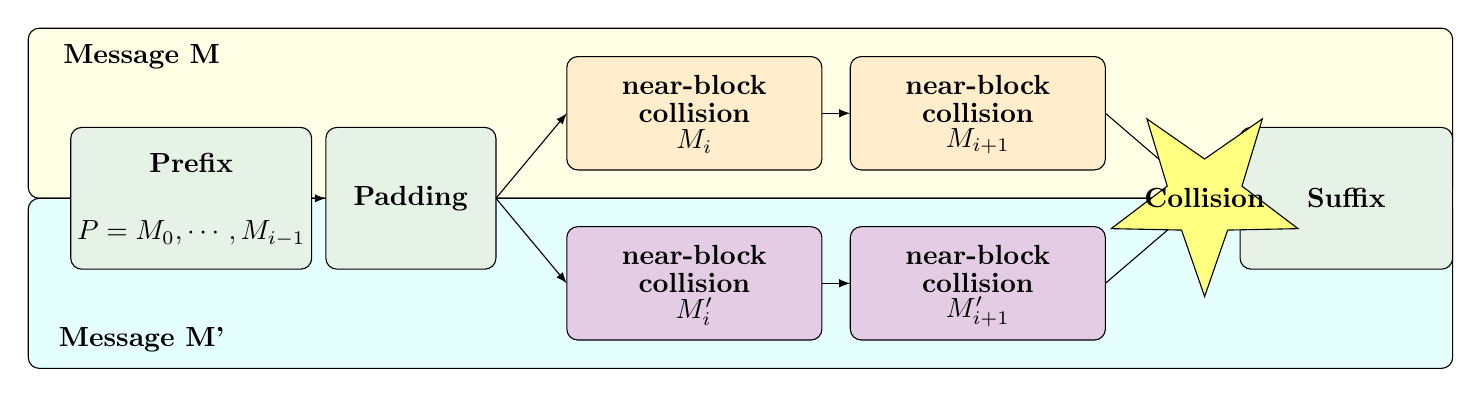
\begin{tikzpicture}[scale=1.8]

          \draw  [rounded corners, fill=Yellow!10] (-0.3,4) rectangle (9.75,5.2);
          \node [align=center] at (0.5,5){\textbf{Message M}};

          \draw  [rounded corners,fill=Cyan!10] (-0.3,2.8) rectangle (9.75,4);
          \node [align=center] at (0.5,3){\textbf{Message M'}};
        %Box Messages
          \draw  [rounded corners,fill=Green!10] (0,3.5) rectangle (1.7,4.5);
          \node [align=center] at (0.85,4.25){\textbf{Prefix}};
          \node [align=center] at (0.85,3.75){\textbf{$P=M_0,\cdots,M_{i-1}$}};

          \draw  [rounded corners,fill=Green!10] (1.8,3.5) rectangle (3,4.5); \node [align=center] at (2.40,4){\textbf{Padding}};
          
          \draw  [rounded corners,fill=Orange!20] (3.5,4.2) rectangle (5.3,5);
          \node [align=center] at (4.4,4.8){\textbf{near-block}};
          \node [align=center] at (4.4,4.6){\textbf{collision}};
          \node [align=center] at (4.4,4.4){\textbf{$M_i$}};

          \draw  [rounded corners,fill=Purple!20] (3.5,3) rectangle (5.3,3.8);
          \node [align=center] at (4.4,3.6){\textbf{near-block}};
          \node [align=center] at (4.4,3.4){\textbf{collision}};
          \node [align=center] at (4.4,3.2){\textbf{$M'_i$}};

          \draw  [rounded corners,fill=Orange!20] (5.5,4.2) rectangle (7.3,5);
          \node [align=center] at (6.4,4.8){\textbf{near-block}};
          \node [align=center] at (6.4,4.6){\textbf{collision}};
          \node [align=center] at (6.4,4.4){\textbf{$M_{i+1}$}};
          
          \draw  [rounded corners,fill=Purple!20] (5.5,3) rectangle (7.3,3.8);
          \node [align=center] at (6.4,3.6){\textbf{near-block}};
          \node [align=center] at (6.4,3.4){\textbf{collision}};
          \node [align=center] at (6.4,3.2){\textbf{$M'_{i+1}$}};
          
        \draw  [rounded corners,fill=Green!10] (8.25,3.5) rectangle (9.75,4.5);
           \node [align=center] at (9,4){\textbf{Suffix}};
           %Traits et Fleches
         \draw [->, >=latex] (1.7,4) -- (1.8,4);
           
        \draw [->, >=latex] (3,4) -- (3.5,3.4);
        \draw [->, >=latex] (3,4) -- (3.5,4.6);
        
        \draw [->, >=latex] (5.3,3.4) -- (5.5,3.4);
        \draw [->, >=latex] (5.3,4.6) -- (5.5,4.6);
        
        \draw [->, >=latex] (7.3,3.4) -- (8,4);
        \draw [->, >=latex] (7.3,4.6) -- (8,4);

        \node[draw, star, star points=5, star point ratio=.4,fill=Yellow!50]
at (8,4) {\textbf{\textsc{Collision}}};
        \end{tikzpicture}
        \caption{\label{fig:collision-attack}Identical prefix collision attack.}
\end{figure}


\section{Merkle-Damg\r{a}rd Construction Weaknesses}

In addition to the work done on SHA-1 and MD5, which has convinced many cryptographers that these hash functions are no longer secure, the Merkle-Damg\r{a}rd construction itself has severeal inherent weaknesses.
Indeed cryptographic hash functions that rely on this construction are usually assumed to have the three security properties described in Section~\ref{sec:requirements}: collision resistance, preimage resistance, and second preimage resistance. Yet many additional properties are also required of hash functions in practical applications.

Hereafter are a few such requirements that hash functions based on the Merkle-Damg\r{a}rd construction fail to meet:
\begin{itemize}
\item Resistance to \emph{length extension attacks}:
   As demonstrated in Figure~\ref{fig:ExtensionAttack}, due to the incremental structure of the construction, for all $x \in \mathcal{E}$, knowing $H(M_1,M_2,\cdots M_i)$ anyone can calculate  $H(M_1,M_2,\cdots M_i, x)$ without knowing  the values of $M_1,M_2,\cdots M_i$.

  \begin{figure}[ht]
\centering
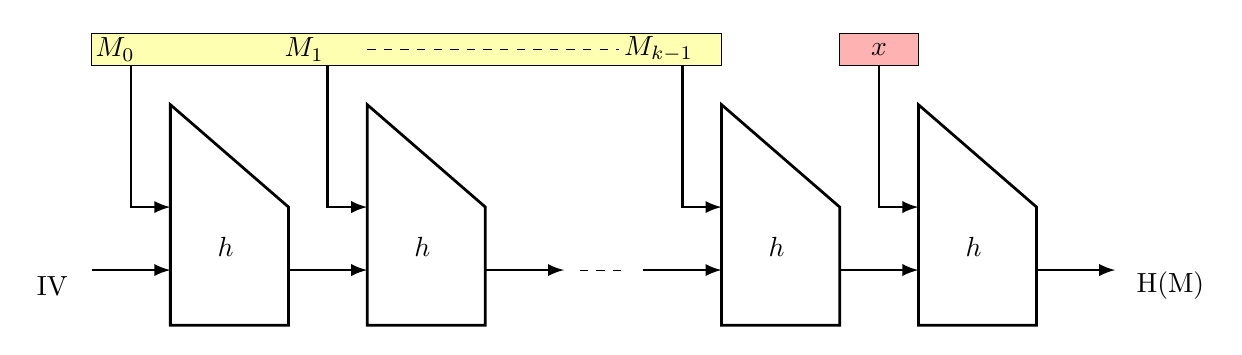
\begin{tikzpicture}

  \draw[fill=Yellow!30] (-1,3.3) rectangle (7,3.7);
  \draw[fill=Red!30] (8.5,3.3) rectangle (9.5,3.7);
\node at (-0.7,3.5){$M_{0}$};
\draw[->, >=latex, line width=1pt] (-0.5,3.3) -- (-0.5,1.5) -- (0,1.5);
\node[align=center] at (-1.5,0.5){IV};
\draw[->, >=latex, line width=1pt] (-1,0.7) -- (0,0.7);
\draw[line width=1pt] (0,0) -- (0,2.8) -- (1.5,1.5) -- (1.5,0) -- cycle;
\node at(0.7,1){$h$};

\node at (1.7,3.5){$M_{1}$};
\draw[->, >=latex, line width=1pt] (2,3.3) -- (2,1.5) -- (2.5,1.5);
\draw[->, >=latex, line width=1pt] (1.5,0.7) -- (2.5,0.7);
\draw[line width=1pt] (2.5,0) -- (2.5,2.8) -- (4,1.5) -- (4,0) -- cycle;
\node at(3.2,1){$h$};
\draw[->, >=latex, line width=1pt] (4,0.7) -- (5,0.7);

\draw[dashed] (5.2,0.7) -- (5.8,0.7);
\draw[dashed] (2.5,3.5) -- (5.7,3.5);

\node at (6.2,3.5){$M_{k-1}$};
\draw[->, >=latex, line width=1pt] (6.5,3.3) -- (6.5,1.5) -- (7,1.5);
\draw[->, >=latex, line width=1pt] (6,0.7) -- (7,0.7);
\draw[line width=1pt] (7,0) -- (7,2.8) -- (8.5,1.5) -- (8.5,0) -- cycle;
\node at(7.7,1){$h$};

\node at (9,3.5){$x$};
\draw[->, >=latex, line width=1pt] (9,3.3) -- (9,1.5) -- (9.5,1.5);
\draw[->, >=latex, line width=1pt] (8.5,0.7) -- (9.5,0.7);
\draw[line width=1pt] (9.5,0) -- (9.5,2.8) -- (11,1.5) -- (11,0) -- cycle;
\node at(10.2,1){$h$};
\draw[->, >=latex, line width=1pt] (11,0.7) -- (12,0.7);
\node[align=center] at (12.7,0.5){H(M)};

\end{tikzpicture}
\caption{\label{fig:ExtensionAttack}Extension attack against the Merkle-Damg\r{a}rd construction.}
\end{figure}

\item Resistance to \emph{multi-collision attacks}:
  \begin{defn}Given a hash function H, a \emph{ multi-collision or r-multi-collision attack} finds many messages with the same hash value, ie: $r$ messages $\{ M^{(1)} \cdots M^{(r)}\}$,  such that $H(M^{(1)} )= H(M^{(2)})= \cdots H(M^{(r)})$.
  \end{defn}
  It has been proven by Antoine Joux~\cite{MC04} that finding multicollisions on iterated hash functions based on the Merkle-Damg\r{a}rd construction is not much harder than finding ordinary collisions.

\item Resistance to \emph{herding attacks}~\cite{HH06}:
  \begin{defn} In a \emph{herding attack}, the adversary first commits to a hash value and is then provided with a prefix. The attacker is required to find a suitable suffix that “herds” to the previously committed hash value. That is, given $x$, $h$, and a hash function $H$, the adversary must find $y$ such that $H(x\vert \vert y)=h$.

    A hash function that resists to herding attacks is said to be \emph{Chosen Target Forced Prefix (CTFP) preimage resistant}.
  \end{defn}
\end{itemize}

\vspace{.5cm}

 These vulnerabilities of the Merkle-Damg\r{a}rd construction emphasize the opinion that the next generation of hashing algortithms to be standardised and widely deployed must rely on a fundamentally new underlying structure. 


%% PART 3
\chapter{Cryptographic Sponge Functions}\label{chap:Sponge}
The SHA-2 family of functions is still considered cryptographically secure. However advances in hash function analysis threaten these crypto-systems, and as they all rely on the same underlying construction, a potential breakthrough in their cryptanalysis could break them all. Moreover selecting and implementing a new standard for all protocols that use cryptographic hashes is a slow process. This is why a new family of hash functions has been standardised: the SHA-3 family of functions, approved by the NIST in August 2015. This additional family provides resiliance against future advances in hash function analysis, as it relies on a fundamentally different design pattern: the \emph{sponge construction}.
Thus even if hash functions based on the Merkle-Damg\r{a}rd construction are broken, the SHA-3 family of functions will be at hand to replace them.

A \emph{cryptographic sponge function} is a function which uses the \emph{sponge construction} structure. This structure is defined in Section~\ref{sec:Sponge}, we then describe the standardised implementation of such sponge functions: the SHA-3\footnote{Secure Hash Algorithm-3} family.

\section{Definitions: Random Oracles, Transformations and Permutations}
We denote a random oracle by $\mathcal{RO}$.
\begin{defn} A random oracle $\mathcal{RO}$ takes as input binary strings of any length and returns for each input a random infinite string, i.e., it is a map from $\mathbb{Z}_2^∗$ to $\mathbb{Z}_2^{\infty}$, chosen by selecting each bit of $\mathcal{RO}(M)$ uniformly and independently, for every $M$.
\end{defn}
A $\mathcal{RO}$ whose output is truncated to its $l$ first bits is denoted $Z = \mathcal{RO}(M, l)$. 
We also need the concept of a random (fixed-width) transformation.
\begin{defn} A \emph{random transformation} with given width $b$ is a transformation drawn randomly and uniformly from the set of all $2^{b\cdot 2^b}$ b-bit transformations.
\end{defn}
Finally, we define a random (fixed-width) permutation.
\begin{defn} A \emph{random permutation} with given width $b$ is a permutation drawn randomly and uniformly from the set of all $2^b\!$ b-bit permutations.
\end{defn}

\section{Construction}\label{sec:Sponge}
\subsection{Outline}
The sponge construction is a simple iterated construction for building a function F with \emph{variable-length input and arbitrary output length} based on a \textbf{fixed-length transformation or permutation $f$} operating on a fixed number $b$ of bits. Here $b$ is called \textbf{the width}.

The sponge construction operates on a state of $b = r + c$ bits. The value $r$ is called \textbf{the bitrate} and the value \textbf{$c$ the capacity}.

First, all the bits of the state are initialized to zero. The input message is padded and cut into blocks of $r$ bits. 

The sponge construction then proceeds in two phases: the absorbing phase, during which all message blocks are processed, followed by the squeezing phase, which outputs the number of output blocks chosen by the user.


\subsection{The Sponge Construction}\label{section:sponge}
The sponge construction builds a function \textsc{sponge}[$f$,pad,r]: $\mathbb{Z}_2^∗ \rightarrow \mathbb{Z}_2^\infty$ using:
\begin{itemize}[label=\textperiodcentered,nolistsep]
\item a fixed-length transformation or permutation $f{\{0,1\}}^b \rightarrow {\{0,1\}}^b$
\item a sponge-compliant padding rule “pad”
\item and a parameter \textbf{bitrate} $r$.
\end{itemize}
A finite-length output can be obtained by truncating it to its $l$ first bits. We call an instance of the sponge construction a \textbf{sponge function}.

The transformation or permutation $f$ operates on a fixed number of bits, the \textbf{width $b$}. The sponge construction has a \textbf{state} of $b$ bits. 

First, all the bits of the state are initialized to zero. The input message is padded and cut into $r$-bits blocks. Then it proceeds in two phases: the \emph{absorbing phase} followed by the \emph{squeezing phase}. During both these phases we distinguish the first $r$ bits of the state, called the \textbf{outer part} and denoted \textbf{$\overline{s}$}, from the remaining $b − r$ bits of the stated, called the \textbf{inner state $\widehat{s}$}. These two parts of the state will be treated differently by the sponge construction.  The inner state is of length $b − r$ and is called the \textbf{capacity c}. 

The two phases are:
\begin{itemize}
\item \textbf{Absorbing phase}: The $r$-bit input message blocks are XORed into the outer part $\overline{s}$ of the state, interleaved with applications of the function $f$. When all message blocks are processed, the sponge construction switches to the squeezing phase.

\item \textbf{Squeezing phase}: The outer part of the state is iteratively returned as output blocks, inter-leaved with applications of the function $f$. The number of iterations is determined by the desired number of bits $l$.
\end{itemize}

Finally the output is truncated to its first $l$ bits. The $c$-bit inner state is never directly affected by the input blocks and never output during the squeezing phase. The capacity $c$ actually determines the attainable security level of the construction. We use the term \emph{random sponge} to denote a sponge function with $f$ a random transformation or permutation.

The sponge construction is illustrated in Figure~\ref{fig:sponge}, and Algorithm~\ref{algo:sponge} provides a formal definition.

In this representation the state is a binary string of a given length $b$ and the message blocks are $r$-bit strings.

\begin{figure}[H]
\centering
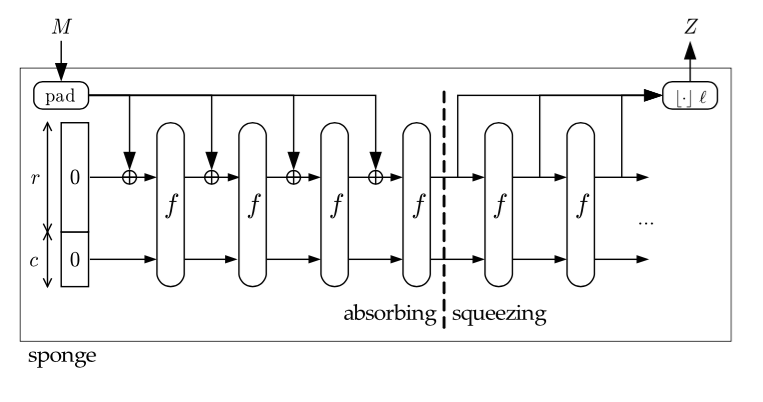
\includegraphics[scale=0.5]{img/sponge1.png}
\caption{\label{fig:sponge}The sponge construction $Z = \textsc{sponge}\lbrack f , pad, r\rbrack (M, l)$}
\end{figure}


\begin{algorithm}[H]
\caption{The sponge construction \textsc{sponge}[f, pad, r] (M,l)}
\label{algo:sponge}

\begin{algorithmic}[1]
\Require{$r < b$}

\Ensure{$Z = sponge(M, l)$ with $M \in \mathbb{Z}_2^∗$, $l \in \mathbb{N}^{*+}$ and $Z ∈ \mathbb{Z}_2^l$}

\State{$P = M\vert \vert pad\lbrack r\rbrack (\vert M\vert )$ }
\State{$s = 0^b$}

\For{$i \gets 0$ to $\vert P\vert_r − 1$ }
\State{$s = s \oplus (P_i\vert \vert0^{b−r})$}
\State{$s = f(s)$}
\EndFor{}

\State{$Z = \lfloor s\rfloor_r$}

\While{$\vert Z\vert_r \times r < l$}
\State{$s = f(s)$}
\State{$Z = Z\vert \vert \lfloor s\rfloor _r$ }
\EndWhile{}

\Return{$\lfloor Z\rfloor _l$}
\end{algorithmic}
\end{algorithm}


\subsection{Auxiliary Functions}\label{section:aux}
In this section we introduce two additional functions \textsc{absorb} and \textsc{squeeze} which represent the two phases of the sponge function introduced above. These will help in the understanding of attacks on the sponge function.


The absorbing function \textsc{absorb}[f, r] takes as input a string $P$ with $\vert P\vert$ multiple of $r$ and returns the value of the state after absorbing P. The absorbing function is defined in Algorithm~\ref{algo:absorb}.

\begin{algorithm}[H]
\caption{The absorbing function \textsc{absorb}[f, r]}
\label{algo:absorb}
\begin{algorithmic}[1]
\Require{$r < b$}
\Ensure{$s=absorb(P)$ with $P \in \mathbb{Z}_2^∗$ and $s \in \mathbb{Z}_2^b$}

\State{$s = 0^b$}

\For{$i = 0$ to $\vert P\vert_r − 1$}
\State{$s = s \oplus (P_i\vert \vert0^{b−r})$}
\State{$s = f(s)$ }
\EndFor{}

\Return{$s$}
\end{algorithmic}
\end{algorithm}

The squeezing function \textsc{squeeze}[f, r] takes as input a state $s$ and a positive integer $l$. This function returns the output truncated to $l$ bits of the sponge function with $s$ the state at the beginning of the squeezing phase. The squeezing function is defined in Algorithm~\ref{algo:squeeze}.

\begin{algorithm}[H]
\caption{The squeezing function \textsc{squeeze}[f, r]}
\label{algo:squeeze}

\begin{algorithmic}[1]
\Require{$r < b$}

\Ensure{$Z=squeeze(s,l)$ with $s \in \mathbb{Z}_2^b$, $l \in \mathbb{N}^{*+}$ and $Z \in \mathbb{Z}_2^l$}

\State{$Z = \lfloor s\rfloor_r$}


\While{$\vert Z\vert_r \times r< l$}
\State{$s = f(s)$}
\State{$Z = Z\vert \vert \lfloor s\rfloor _r$ }
\EndWhile{}

\Return{$\lfloor Z\rfloor _l$}

\end{algorithmic}
\end{algorithm}


\begin{defn}
$P$ is a \emph{path to the state} $s$ if $s = absorb(P)$.
\end{defn}

Clearly \textsc{absorb}[f, r]$($empty string$) = 0^b$. In general, the $j$-th block of the output of a sponge function corresponding to an input $M$ is equal to:
\begin{equation}
Z_j = \overline{\textsc{absorb}[f, r]}(P\vert \vert 0^{rj})\mbox{, } j \ge 0,
\end{equation}
with $P = M\vert \vert pad\lbrack r\rbrack (\vert M\vert)$.

Indeed, the for loop of \textsc{absorb}[f, r] will be ran $\vert P\vert_r +1$ times to $P\vert \vert 0^{rj}$. However for the last $j$ iterations of the loop, the \textsc{xor}ing of the input message blocs with the state will have no effect, as for $i\ge \vert P\vert_r$, $M_i=0^r$. Thus each iteration for $i\ge \vert P\vert_r$ only applies $f$  to the state, which is what the squeezing phase does.

Alternatively, the absorbing function can be used to express the states that the sponge traverses both as it absorbs an input M and as it is being squeezed. The traversed states are $absorb(P')$ for any $P'$ prefix of $P\vert \vert 0^\infty$, with $P = M\vert \vert pad\lbrack r\rbrack (\vert M\vert )$, including the empty string.

\subsection{Generic Primary Attacks On A Sponge Function}

The attacks hereby described are \emph{generic attacks}. For sponge functions we define it as follows: 

\begin{defn}
An attack on a sponge function is a generic attack if it does not exploit specific properties of $f$.
\end{defn}

We call \emph{primary attacks}, attacks that would not apply to $\mathcal{RO}$'s as they have no concept of state, but will apply to sponge functions due to their finite state.

These concepts are fundamental as they introduce upper-bounds to the security of any real sponge function.

As seen previously, the sponge function can be seen as the subsequent application of a padding rule, the \textsc{absorb} function and the \textsc{squeeze} function.

\begin{nota}
If $Z=$\textsc{sponge}$\lbrack f$, pad,$r\rbrack(M,l)$, we call:
\begin{equation}
\begin{aligned}
P & = M\vert \vert pad \lbrack r \rbrack (\vert M \vert )  \\
s & = \mbox{\textsc{absorb}} \lbrack f,r \rbrack (P) \\
Z & = \mbox{\textsc{squeeze}} \lbrack f,r \rbrack (s,l) \\
\end{aligned}
\end{equation}
\end{nota}
Let us consider the cryptographic requirements of a hashing function:
\subsubsection{Cryptographic resistance of the absorb function}
It is in general difficult to find a pre-image to either of the auxiliary functions introduced in Section~\ref{section:aux} i.e.\ it is difficult to find a path $P$ to a given state $s$, and it is difficult to find the state $s$ for a given output $Z$.

\begin{defn}
A \emph{state collision} is a pair of different paths $P \ne Q$ to the same state: \textsc{absorb} ($P$) = \textsc{absorb} ($Q$).
\end{defn}
It is generally hard to find two paths leading to the same state. It is therefore also difficult to find a pre-image to the \textsc{absorb} function i.e.\ it is difficult to find a path $P$ to a given state $s$.

\paragraph{Consequences of state collision}
If a state collision is obtained during the absorbing phase, an overall collision for the sponge function is easily obtainable.
If \textsc{absorb} ($P$) = \textsc{absorb} ($Q$) then the squeezing part will produce the same output values for \textsc{absorb} ($P\vert \vert 0^{rj}$) = \textsc{absorb} ($Q\vert \vert 0^{rj}$) for all j.

A state collision can also lead to a periodical output if $\exists d$ such that \textsc{absorb} ($P$) = \textsc{absorb} ($P\vert \vert 0^{rd}$). The periodicity would then be of $d$ output blocks (since $s_{\vert M\vert_r + j} = \textsc{absorb}(P\vert \vert 0^{rj})$).


\begin{defn}
An \emph{inner collision} is a pair of different paths $P \ne Q$ to the same inner state:
$\widehat{\textsc{absorb}}(P) = \widehat{\textsc{absorb}}(Q)$.
\end{defn}

Clearly a state collision implies an inner collision, and as explained below, a state collision can easily be obtained from an inner collision.

If we have an inner collision $\widehat{\textsc{absorb}}(P) = \widehat{\textsc{absorb}}(Q)$, then for any $A,B \in \mathbb Z_2^r$ that verify $\overline{\textsc{absorb}}(P)\oplus A = \overline{\textsc{absorb}}(Q) \oplus B$, the paths $P\vert \vert A$ and $Q \vert \vert B$ will lead to a state collision.

\subsubsection{Cryptographic resistance of the squeeze function}
In general it is hard to find a state s such that $\textsc{squeeze}(s, \vert Z\vert ) = Z$ for long strings Z. Depending on the origin of Z and the goal of the adversary, we distinguish two cases: 
\begin{itemize}[label=\textperiodcentered,nolistsep]
\item \emph{output binding}: Z is not necessarily the result of the squeezing of the state and so there may be no solution.
\item \emph{state recovery}: Z has been obtained by the squeezing of a state s.
\end{itemize}
Let us define these two problems formally:
\begin{defn}
Given an arbitrary string Z, \emph{output binding} is finding a state s such that $\textsc{squeeze}(s, \vert Z\vert ) = Z$.
\end{defn}
The expected number of states that squeeze to a given string $Z$ is $2^{b−\vert Z\vert}$. If $\vert Z\vert  > b$, the probability that such a state exists is $\approx 2^{b−\vert Z\vert }$.

\begin{defn}
State recovery is finding a state s, given a string Z with $Z = \textsc{squeeze}(s, \vert Z\vert )$.
\end{defn}


If $\vert Z\vert > b$, it is likely that there is only a single solution and that output binding results in recovery of the unique state that it was squeezed from. If $\vert Z \vert \le b$ there are typically several states that squeeze to $Z$ and output binding does not necessarily result in state recovery.

\section{Keccak-p Permutations}
\textsc{Keccak}-p is a fixed length permutation which is the underlying permutation (denoted earlier by $f$) used by the \textsc{sha-3} family of functions as specified by the NIST~\cite{NIST}. The steps of this permutation are described below, before defining the hash functions in their entirety in Section~\ref{section:sha3}.

\begin{defn} Two parameters are specified for a \textsc{Keccak}-p function:
  \begin{itemize}[label=\textperiodcentered,nolistsep]
  \item The \emph{width} of a permutation is the fixed length of the bit strings that are permuted.
    \item A \emph{round} is an iteration of an internal transformation.
  \end{itemize}
\end{defn}

For any $b$ in $ \{25, 50, 100, 200, 400, 800, 1600\} $ and any positive integer $n_r$, \textsc{Keccak}-p $\lbrack b, n_r \rbrack$ denotes the \textsc{Keccak}-p permutation of \emph{width} $b$ with $n$ \emph{rounds}.

A round of a \textsc{Keccak}-p permutation, denoted by \textsc{Rnd}, consists of a sequence of five transformations, called the \emph{step mappings}. The permutation is specified in terms of the values of the state. The state is initially set to the
input values of the permutation.
\subsection{The State}
For the sake of simplicity and to help understanding we shall limit our study to the case where $b=50$.
The NIST standard specifies two other quantities related to $b$: $w=b/25$ and $l = \log_2{b/25}$. In our case $l = 1$ and $w=2$.

The state of the \textsc{Keccak}-p permutation can be represented either:
\begin{itemize}
\item as a string whose bits are indexed from 0 to $b-1$. $S=S\lbrack 0 \rbrack \vert \vert S\lbrack 1 \rbrack \vert \vert S\lbrack 2 \rbrack \vert \vert \cdots S\lbrack b-1 \rbrack$
\item as a \emph{state array} which is a three dimensional array representation of the state \textbf{A}. A is a 5-by-5-by-$w$ array of bits. And $A\lbrack x,y,z \rbrack$ corresponds to the bit $(x,y,z) \in \llbracket 0,5 \llbracket \times \llbracket 0,5 \llbracket \times \llbracket 0,w \llbracket$.
\end{itemize}
In figure~\ref{fig:StateArray}, the different parts of a \textsc{Keccak}-p permutation state array are represented.

The two-dimensional parts of the array are called \emph{sheets}, \emph{planes} and \emph{slices}.

The single-dimensional parts of the array are called \emph{rows}, \emph{columns}, and \emph{lanes}.

\begin{figure}[H]
\centering
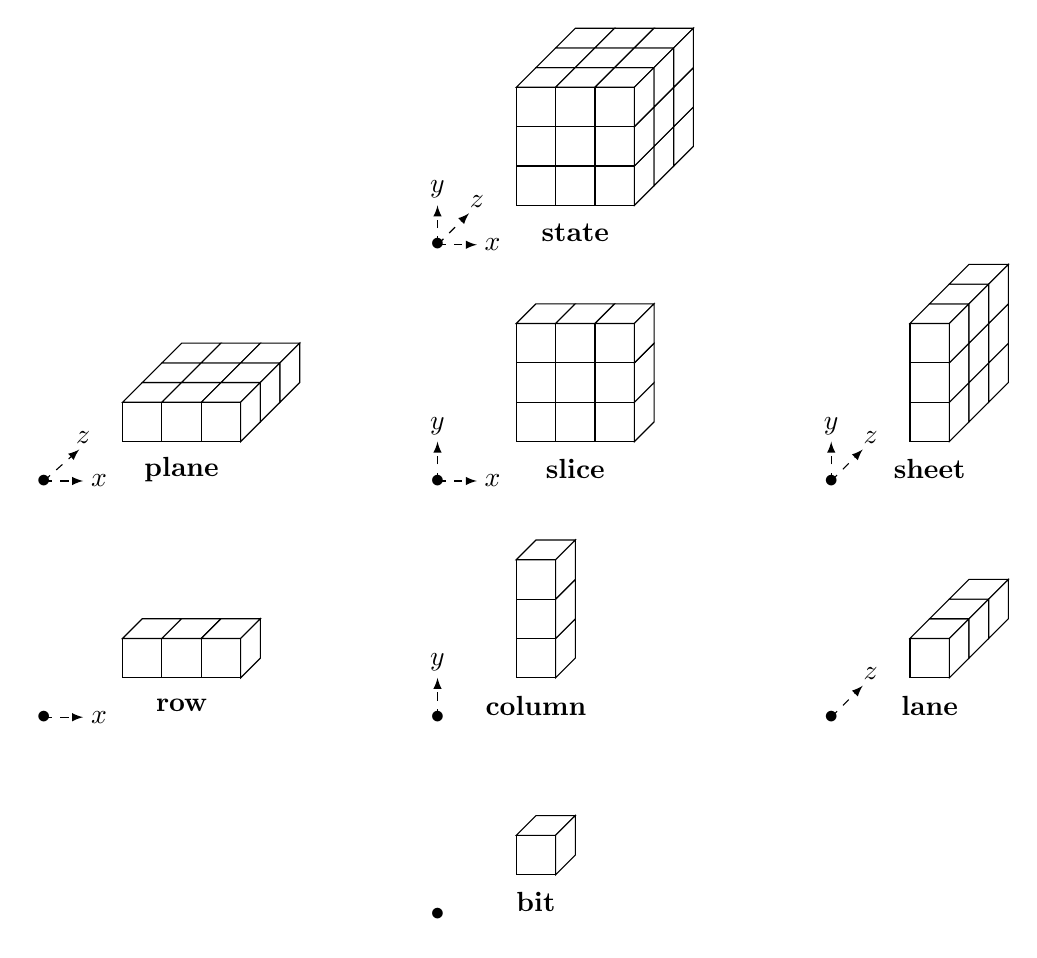
\begin{tikzpicture}[scale=0.5]

\newcommand\xaxis{1}
\newcommand\yaxis{1}
\newcommand\zaxis{1}
  
\newcommand\faceside[6]{
  \draw (-2+#4,-1+#5) node[]{} node{$\bullet$};
  \pgfmathparse{#1/2+#4}
  \node[text centered, font=\bf] at (\pgfmathresult,-0.7+#5) {#6};
  \foreach \a in {1,...,#1} {
    \foreach \b in {1,...,#2} {
      \fill[fill=white, draw=black] (#4+-1+\a,#5+-1+\b) -- (#4+\a,#5+-1+\b) -- (#4+\a,#5+\b) -- (#4+-1+\a,#5+\b) -- cycle;
    }
    \pgfmathparse{-1+#3}
    \foreach \d [evaluate=\d as \dd using \d*0.5] in {0,...,\pgfmathresult} {
      \fill[fill=white, draw=black] (#4+-1+\a+\d-\dd,#5+#2+\d-\dd) -- (#4+\a+\d-\dd,#5+#2+\d-\dd) -- (#4+\a+\d+0.5-\dd,#5+#2+\d+0.5-\dd) -- (#4+\a+\d-0.5-\dd,#5+#2+\d+0.5-\dd) -- cycle;
    }
  }
  \foreach \c in {1,...,#2} {
    \pgfmathparse{-1+#3}
    \foreach \e [evaluate=\e as \ee using \e*0.5] in {0,...,\pgfmathresult} {
      \fill[fill=white, draw=black] (#4+#1+\e-\ee,#5+-1+\c+\e-\ee) -- (#4+#1+\e+0.5-\ee,#5+-1+\c+\e+0.5-\ee) -- (#4+#1+\e+0.5-\ee,#5+0.5+\c+\e-\ee) -- (#4+#1+\e-\ee,#5+\c+\e-\ee) -- cycle;
      }
  }
}

\faceside{1}{1}{1}{10}{0}{bit}
\faceside{3}{1}{1}{0}{5}{row}\draw [->, >=latex, dashed] (-2,4) -- (-1,4);\draw (-0.6,4) node[]{$x$};
\faceside{1}{3}{1}{10}{5}{column}\draw [->, >=latex, dashed] (8,4) -- (8,5);\draw (8,5.4) node[]{$y$};
\faceside{1}{1}{3}{20}{5}{lane}\draw [->, >=latex, dashed] (18,4) -- (18.8,4.8);\draw (19,5.1) node[]{$z$};
\faceside{3}{1}{3}{0}{11}{plane}\draw [->, >=latex, dashed] (-2,10) -- (-1,10);\draw [->, >=latex, dashed] (-2,10) -- (-1.1,10.8);\draw (-0.6,10) node[]{$x$};\draw (-1,11.1) node[]{$z$};
\faceside{3}{3}{1}{10}{11}{slice}\draw [->, >=latex, dashed] (8,10) -- (9,10);\draw [->, >=latex, dashed] (8,10) -- (8,11);\draw (9.4,10) node[]{$x$};\draw (8,11.4) node[]{$y$};
\faceside{1}{3}{3}{20}{11}{sheet}\draw [->, >=latex, dashed] (18,10) -- (18,11);\draw [->, >=latex, dashed] (18,10) -- (18.8,10.8);\draw (18,11.4) node[]{$y$};\draw (19,11.1) node[]{$z$};
\faceside{3}{3}{3}{10}{17}{state}\draw [->, >=latex, dashed] (8,16) -- (9,16);\draw [->, >=latex, dashed] (8,16) -- (8,17);\draw [->, >=latex, dashed] (8,16) -- (8.8,16.8);\draw (9.4,16) node[]{$x$};\draw (8,17.4) node[]{$y$};\draw (9,17.1) node[]{$z$};

\end{tikzpicture}
\caption{\label{fig:StateArray}The parts of the state array for $x,y,z \in\llbracket 0,3 \llbracket \times \llbracket 0,3 \llbracket \times \llbracket 0,3 \llbracket$ }
\end{figure}

We shall label our state arrays in such a way that the lane that corresponds to (x,y) = (0,0) is in the center of the slices, as in~\ref{fig:LabelStateArray}

\begin{figure}[H]
\centering
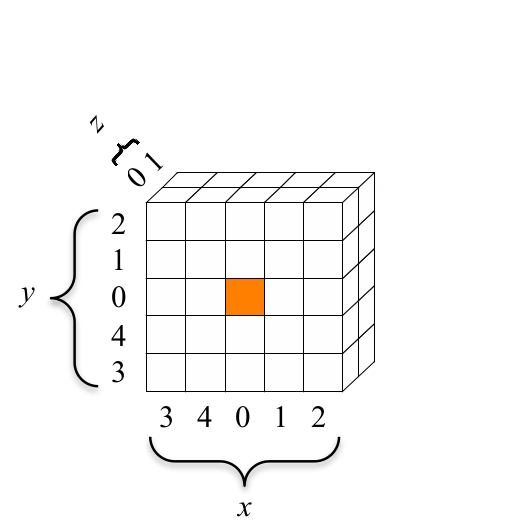
\includegraphics[width=0.5\textwidth]{img/LabelStateArray.png}
\caption{\label{fig:LabelStateArray}Convention for the coordinates of the state array.}
\end{figure}

The correspondance between the string reprsentation of the state and the state array is defined as follows:

For $(x,y,z) \in \llbracket 0,5 \llbracket \times \llbracket 0,5 \llbracket \times \llbracket 0,w \llbracket$,
$$A\lbrack x,y,z \rbrack=S\lbrack w\cdot (5y+x)+z \rbrack.$$



In our example $b=50$, therefore $w=2$, which gives us:
$$A\lbrack x,y,z \rbrack=S\lbrack 2\cdot (5y+x)+z \rbrack.$$

\begin{equation}
\begin{aligned}
A \lbrack 0,0,0\rbrack = S\lbrack 0 \rbrack & \hspace{2cm} A \lbrack 1,0,0\rbrack = S\lbrack 2 \rbrack & \hspace{2cm} \ldots & \hspace{2cm} A \lbrack 4,0,0\rbrack = S\lbrack 8 \rbrack\\
A \lbrack 0,0,1\rbrack = S\lbrack 1 \rbrack & \hspace{2cm} A \lbrack 1,0,1\rbrack = S\lbrack 3 \rbrack & \hspace{2cm} \ldots & \hspace{2cm} A \lbrack 4,0,1\rbrack = S\lbrack 9 \rbrack\\
\end{aligned}
\end{equation}

and

\begin{equation}
\begin{aligned}
A \lbrack 0,1,0\rbrack = S\lbrack 10 \rbrack & \hspace{2cm} A \lbrack 1,1,0\rbrack = S\lbrack 12 \rbrack & \hspace{2cm} \ldots & \hspace{2cm} A \lbrack 4,1,0\rbrack = S\lbrack 18 \rbrack\\
A \lbrack 0,1,1\rbrack = S\lbrack 11 \rbrack & \hspace{2cm} A \lbrack 1,1,1\rbrack = S\lbrack 13 \rbrack & \hspace{2cm} \ldots & \hspace{2cm} A \lbrack 4,1,1\rbrack = S\lbrack 19 \rbrack\\
\vdots                                       & \hspace{2cm} \vdots                                       & \hspace{2cm} \vdots & \hspace{2cm} \vdots                                    \\
A \lbrack 0,4,0\rbrack = S\lbrack 40 \rbrack & \hspace{2cm} A \lbrack 1,4,0\rbrack = S\lbrack 42 \rbrack & \hspace{2cm} \ldots & \hspace{2cm} A \lbrack 4,4,0\rbrack = S\lbrack 48 \rbrack\\
A \lbrack 0,4,1\rbrack = S\lbrack 41 \rbrack & \hspace{2cm} A \lbrack 1,4,1\rbrack = S\lbrack 43 \rbrack & \hspace{2cm} \ldots & \hspace{2cm} A \lbrack 4,4,1\rbrack = S\lbrack 49 \rbrack\\
\end{aligned}
\end{equation}


The reverse operation, i.e.\ converting a state array representation to the string representation can be done using the lanes and planes of A.

Bits in a given lane follow sequencial order ($x=x, y=y, z=z+1$), and at the end of a lane, the following indexation of S if obtained by moving to the next lane in the same plane ($x=x+1, y=y, z=0$).
Once all the lanes in a plane have been explored, the following indexation of S if obtained by moving to the first lane of the next plane ($x=0, y=y+1, z=0$).

\begin{defn}
For $(x,y) \in \llbracket 0,5 \llbracket \times \llbracket 0,5 \llbracket$, the string \textbf{Lane (x,y)} is defined as:
$$Lane (x, y) = A\lbrack x, y, 0\rbrack \vert \vert A\lbrack x, y, 1\rbrack \vert \vert A\lbrack x, y, 2\rbrack \vert \vert \cdots \vert \vert A\lbrack x, y, w-2\rbrack \vert \vert A\lbrack x, y, w-1\rbrack $$
\end{defn}
In our example:
\begin{equation}
\begin{aligned}
Lane (0, 0) =& A\lbrack 0, 0, 0\rbrack \vert \vert A\lbrack 0, 0, 1\rbrack \\
Lane (1, 0) =& A\lbrack 1, 0, 0\rbrack \vert \vert A\lbrack 1, 0, 1\rbrack \\
Lane (2, 0) =& A\lbrack 2, 0, 0\rbrack \vert \vert A\lbrack 2, 0, 1\rbrack \\
\vdots & \\
\end{aligned}
\end{equation}

\begin{defn}
For $ y \in \llbracket 0,5 \llbracket$, the string \textbf{Plane(y)} is defined as:
$$Plane (y) = Lane (0,y) \vert \vert Lane (1,y) \vert \vert Lane (2,y) \vert \vert Lane (3,y) \vert \vert Lane (4,y) $$
\end{defn}
And then
$$S= Plane (0) \vert \vert  Plane (1) \vert \vert Plane (2) \vert \vert  Plane (3) \vert \vert  Plane (4) $$

In our example:
\begin{equation}
\begin{aligned}
S = & A\lbrack 0, 0, 0\rbrack \vert \vert A\lbrack 0, 0, 1\rbrack \\
    & A\lbrack 1, 0, 0\rbrack \vert \vert A\lbrack 1, 0, 1\rbrack \\
    & A\lbrack 2, 0, 0\rbrack \vert \vert A\lbrack 2, 0, 1\rbrack \\
    & A\lbrack 3, 0, 0\rbrack \vert \vert A\lbrack 3, 0, 1\rbrack \\
    & A\lbrack 4, 0, 0\rbrack \vert \vert A\lbrack 4, 0, 1\rbrack \\
    & \\
    & A\lbrack 0, 1, 0\rbrack \vert \vert A\lbrack 0, 1, 1\rbrack \\
    & A\lbrack 1, 1, 0\rbrack \vert \vert A\lbrack 1, 1, 1\rbrack \\
    & A\lbrack 2, 1, 0\rbrack \vert \vert A\lbrack 2, 1, 1\rbrack \\
    & A\lbrack 3, 1, 0\rbrack \vert \vert A\lbrack 3, 1, 1\rbrack \\
    & A\lbrack 4, 1, 0\rbrack \vert \vert A\lbrack 4, 1, 1\rbrack \\
    & \vdots \\
    & A\lbrack 0, 4, 0\rbrack \vert \vert A\lbrack 0, 4, 1\rbrack \\
    & A\lbrack 1, 4, 0\rbrack \vert \vert A\lbrack 1, 4, 1\rbrack \\
    & A\lbrack 2, 4, 0\rbrack \vert \vert A\lbrack 2, 4, 1\rbrack \\
    & A\lbrack 3, 4, 0\rbrack \vert \vert A\lbrack 3, 4, 1\rbrack \\
    & A\lbrack 4, 4, 0\rbrack \vert \vert A\lbrack 4, 4, 1\rbrack \\
\end{aligned}
\end{equation}

\subsection{Step Mappings}
A round of \textsc{Keccak}-p$\lbrack b, n_r \rbrack$ is composed of five step mappings whose algorithms we shall develop below. They all take as input a state array A and output an updated state array. The last step mapping has an additional parameter which is the round index $i_r$.

\subsubsection{The First Step Function $\Theta$}
\begin{algorithm}[H]
\caption{$\Theta$ (A)}
\label{algo:Theta}
\begin{algorithmic}[1]
\For{$(x,z) \in \llbracket 0,5 \llbracket \times \llbracket 0,w \llbracket$}
\State{$C\lbrack x,z\rbrack = A\lbrack x, 0, z\rbrack \oplus A\lbrack x, 1, z\rbrack \oplus A\lbrack x, 2, z\rbrack \oplus A\lbrack x, 3, z\rbrack \oplus A\lbrack x, 4, z\rbrack $}
\EndFor{}

\For{$(x,z) \in \llbracket 0,5 \llbracket \times \llbracket 0,w \llbracket$}
\State{$D\lbrack x,z\rbrack = C\lbrack (x-1) \mod{5}, z\rbrack \oplus C\lbrack (x+ 1) \mod{5}, (z-1) \mod{w}\rbrack $}
\EndFor{}

\For{$(x,y,z) \in \llbracket 0,5 \llbracket \times \llbracket 0,5 \llbracket \times \llbracket 0,w \llbracket$}
\State{$A'\lbrack x, y, z\rbrack = A\lbrack x, y, z\rbrack \oplus D\lbrack x,z\rbrack$}
\EndFor{}

\Return{$A'$}
\end{algorithmic}
\end{algorithm}

Algorithm~\ref{algo:Theta}, which performs the first step mapping, starts by calculating the parity of each column of the state array, to be stored in variables $C\lbrack x,z\rbrack$ for all values of $x$ and $z$.

Then a new set of $5 \times w$ values is computed, each $D\lbrack x,z\rbrack$ representing the sum of the parity of two columns.

Finally each bit in the state is XOR-ed with a value of $D$ as illustrated in Figure~\ref{fig:Theta}.

\begin{figure}[H]
\centering
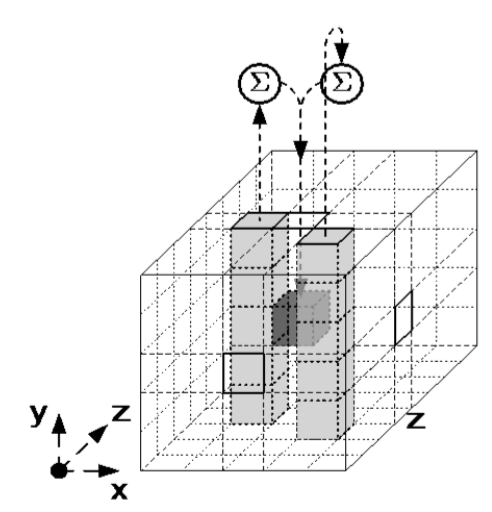
\includegraphics[width=0.3\textwidth]{img/Theta.png}
\caption{\label{fig:Theta}The effect of $\Theta$ on a bit of the state array.}
\end{figure}

\subsubsection{The Second Step Function $\rho$}
$\rho$ rotates each lane by an \emph{offset}, thus each lane is modified by adding the offset to the z coordinate, modulo the lane size $w$. The offset depends on the x and y coordinates of the given lane.
\begin{algorithm}[H]
\caption{$\rho$ (A)}
\label{algo:rho}
\begin{algorithmic}[1]
\For{$z \in \llbracket 0,w \llbracket$}
\State{$A'\lbrack 0, 0, z\rbrack = A\lbrack 0, 0, z\rbrack $}
\EndFor{}
\State{$(x,y) \gets (1,0)$}
\For{$t=0$ to $23$}
\For{$z=0$ to $w-1$}
\State{$A'\lbrack x, y,z\rbrack = A\lbrack x, y, (z-(t+1)\cdot (t+2)/2) \mod{w} \rbrack $}
\EndFor{}
\State{$(x,y) \gets (y, (2\cdot x + 3\cdot y) \mod{5})$}
\EndFor{}
\Return{$A'$}
\end{algorithmic}
\end{algorithm}

\subsubsection{The Third Step Function $\pi$}
$\pi$ rearranges the position of the lanes.
\begin{algorithm}[H]
\caption{$\pi$ (A)}
\label{algo:pi}
\begin{algorithmic}[1]
\For{$(x,y,z) \in \llbracket 0,5 \llbracket \times \llbracket 0,5 \llbracket \times \llbracket 0,w \llbracket$}
\State{$A'\lbrack x, y, z\rbrack = A\lbrack( x+ 3 \cdot y)\mod{5}, x, z\rbrack $}
\EndFor{}
\Return{$A'$}
\end{algorithmic}
\end{algorithm}

\subsubsection{The Third Step Function $\chi$}
$\chi$ XOR's each bit with a non linear function of two other bits in it's row.
\begin{algorithm}[H]
\caption{$\chi$ (A)}
\label{algo:chi}
\begin{algorithmic}[1]
\For{$(x,y,z) \in \llbracket 0,5 \llbracket \times \llbracket 0,5 \llbracket \times \llbracket 0,w \llbracket$}
\Comment{$\cdot$ is equivalent to a boolean AND operation.}
\State{$A'\lbrack x, y, z\rbrack = A\lbrack x, y, z\rbrack \oplus ((A\lbrack( x+ 1)\mod{5}, y, z\rbrack \oplus 1) \cdot A\lbrack (x+2)\mod{5}, y, z\rbrack )$}
\EndFor{}
\Return{$A'$}
\end{algorithmic}
\end{algorithm}

\subsubsection{The Final Step Mapping $\iota$}
The $\iota$ step mapping takes an additional parameter $i_r$ called the \emph{round index}. An auxiliary function $rc$, based on a linear feedback shift register, takes the round index as an input and calculates a \emph{round constant} $RC$. This round constant is then XORed to the \emph{Lane (0,0)} of the state.

\emph{Lane(0,0)} is the only lane that is affected by $\iota$.

\begin{algorithm}[H]
\caption{$rc$ (t)}
\label{algo:rc}
\begin{algorithmic}[1]
\If{$t \mod{255}=0$}
\Return{1}
\EndIf{}
\State{$R \gets 10000000$}
\For{$i=1$ to $t\mod{255}$}
\State{$R \gets 0 \vert \vert R$}
\State{$R\lbrack 0\rbrack \gets R\lbrack 0 \rbrack \oplus \lbrack 8 \rbrack$}
\State{$R\lbrack 4\rbrack \gets R\lbrack 4 \rbrack \oplus \lbrack 8 \rbrack$}
\State{$R\lbrack 5\rbrack \gets R\lbrack 5 \rbrack \oplus \lbrack 8 \rbrack$}
\State{$R\lbrack 6\rbrack \gets R\lbrack 6 \rbrack \oplus \lbrack 8 \rbrack$}
\State{$R=\lfloor R\rfloor _8$}
\EndFor{}
\Return{$R\lbrack 0\rbrack$}
\end{algorithmic}
\end{algorithm}

\begin{algorithm}[H]
\caption{$\iota$ (A, $i_r$)}
\label{algo:iota}
\begin{algorithmic}[1]
\For{$(x,y,z) \in \llbracket 0,5 \llbracket \times \llbracket 0,5 \llbracket \times \llbracket 0,w \llbracket$}
\State{$A'\lbrack x, y, z\rbrack = A\lbrack x, y, z\rbrack$}
\EndFor{}
\For{$j=0$ to $l$}
\State{$RC\lbrack 2^j-1\rbrack = rc(j+7\cdot i_r)$}
\EndFor{}
\For{$z \in \llbracket 0,w \llbracket$}
\State{$A'\lbrack 0, 0, z\rbrack = A'\lbrack 0, 0, z\rbrack \oplus RC\lbrack z \rbrack$}
\EndFor{}
\Return{$A'$}
\end{algorithmic}
\end{algorithm}

\subsection{The Keccak-p Function}
Given a state array A and a round index $i_r$, the round function \textsc{Rnd} is the transformation that results from applying the step mappings $\Theta$, $\rho$, $\pi$, $\chi$, and $\iota$, in that order.
$$\textsc{Rnd}(A,i_r)=\iota ( \chi ( \pi ( \rho (\Theta (A)))), i_r)$$

The $\textsc{Keccak}$-p$\lbrack b, n_r \rbrack$ permutation applies $n_r$ iterations of \textsc{Rnd}.
Algorithm~\ref{algo:keccak} describes the whole permutation, where the input is a bit-string $S$ of length $b$. The width $b$ and number of rounds $n_r$ are fixed parameters.
\begin{algorithm}[H]
\caption{$\textsc{Keccak}$-p$\lbrack b, n_r \rbrack$ (S)}
\label{algo:keccak}
\begin{algorithmic}[1]
  \State{$A \gets S$ converted into a state array}
  \For{$i_r \in \llbracket 12+2\cdot l -n_r, 12 + 2\cdot l -1 \llbracket$}
  \State{$A \gets \textsc{Rnd}(A,i_r)$}
  \EndFor{}
  \State{$S' \gets A$ converted into a bit string of length $b$}
\Return{$S'$}
\end{algorithmic}
\end{algorithm}

\section{SHA-3}\label{section:sha3}
The \textsc{SHA-3} functions are instances of the sponge construction \textsc{sponge}[$f$,pad,r] in which the underlying permutation $f$ is $\textsc{Keccak}$-p$\lbrack b, n_r \rbrack$.

\subsection{Overview}
For all hashing functions in the \textsc{SHA-3} family, the bit-length $b$ is fixed to $1600$ and the number of rounds is set to $24$.

The padding rule used by \textsc{SHA-3} is multi-rate padding, as described in Section~\ref{section:padding}.

This leaves two variable parameters: the desired number of bits $l$ to be output by the sponge construction, and the bitrate $r$.
Seeing as we have $b=r+c=1600$ where $c$ is the capacity, fixing the capacity is equivalent to fixing the bitrate.


The \textsc{SHA-3} family defines six functions, for the different values of the desired digest length and capacity.

Four of these are hash functions (which output a fixed length digest) named \textsc{SHA3}-$l(M)$. The four possible values for $l$ are 224, 256, 384 and 512, and in each case the capacity is fixed to $c=2\times l$. Each of these functions appends a two-bit suffix to the message M.
Thus with the notations used:
$$ \textsc{SHA3}-l(M) =\textsc{sponge}[\textsc{Keccak}-p\lbrack 1600, 24 \rbrack, pad10∗1,1600-2\times l](M\vert \vert 01,l) $$


The two other \textsc{SHA-3} functions are \emph{extendable-output functions}.

\begin{defn}
  An extendable-output function (XOF) is a function on bit strings in which the output can be extended to any desired length.
\end{defn}

\textsc{SHAKE128}$(M,l)$ (for a capacity of 256 bits, and a chosen output length $l$) and SHAKE256 (for a capacity of 512 bits, and a chosen output length $l$) are the first XOFs that NIST has standardized.
Both functions append a four-bit suffix to the message M.
Thus:
\begin{equation}
  \begin{aligned}
    \textsc{SHAKE128}(M,l) & =\textsc{sponge}[\textsc{Keccak}-p\lbrack 1600, 24 \rbrack, pad10∗1,1600-256](M\vert \vert 1111,l) \\
    \textsc{SHAKE256}(M,l) & =\textsc{sponge}[\textsc{Keccak}-p\lbrack 1600, 24 \rbrack, pad10∗1,1600-512](M\vert \vert 1111,l) \\
\end{aligned}
\end{equation}

\subsection{Algorithm And Implementation}
We have chosen to implement \textsc{SHA3}-224.
Therefore our fixed parameters are:
\begin{itemize}[label=\textperiodcentered,nolistsep]
\item Digest length: $l=224$
\item Capacity of the sponge construction: $c=448$
\item Bitrate of the sponge construction: $r=1152$
\item Width of the sponge construction (ie the bit-size of the state): $b=1600$
\item Number of rounds performed by the sponge construction $n_r=24$
\end{itemize}
Thus the resulting hashing algorithm is:
$$ \textsc{SHA3}-224(M) =\textsc{sponge}[\textsc{Keccak}-p\lbrack 1600, 24 \rbrack, pad10∗1,1152](M\vert \vert 01,l) $$

The pseudo-code for the \textsc{SHA3}-224 algorithm is presented in Algorithm~\ref{algo:sha3}.
\begin{algorithm}[H]
\caption{\textsc{SHA3}-224(M)}
\label{algo:sha3}
\begin{algorithmic}[1]
  \State{\textbf{external procedures:} pad10*1, $\textsc{Keccak}$-p$\lbrack b, n_r \rbrack$ }
  \State{$l \gets 224$}
  \State{$n_r \gets 24$}
  \State{$b \gets 1600$}
  \State{$r \gets b-2\times l = 1152$}  \Comment{Set the bitrate r to 1152 bits, ie 144 bytes.}
  \State{$P \gets  M\vert \vert pad10*1\lbrack r\rbrack (\vert M\vert )$}
  \Comment{The padded message length is a multiple of r.}
  \State{$N \gets \vert P \vert_r$}
  \State{Let $P\lbrack n\rbrack$ be the array of strings of length r such that $P=P_0 \vert \vert \ldots \vert \vert P_{N-1}$.}
  \State{$\textsc{ctx} \gets 0^{b}$}

  \For{$i \gets 0$ to $N-1$}
  \State{$\textsc{ctx}\gets \textsc{Keccak}$-p$\lbrack b, n_r \rbrack(\textsc{ctx} \oplus (P_i \vert \vert O^c))$}
  \EndFor{}

\State{$Z = \lfloor \textsc{ctx}\rfloor_r$}

\While{$\vert Z\vert < l$}
\State{$\textsc{ctx}\gets \textsc{Keccak}$-p$\lbrack b, n_r \rbrack(\textsc{ctx})$}
\State{$Z = Z\vert \vert \lfloor \textsc{ctx}\rfloor _r$ }
\EndWhile{}

\Return{$\lfloor Z\rfloor _l$}
\end{algorithmic}
\end{algorithm}


%% CONCLUSION
\begin{frame}<handout:0>
  \frametitle{Plan}
  \tableofcontents[currentsection,subsectionstyle=hide]
\end{frame}

\begin{frame}[fragile]
  \frametitle{Conclusion}

  \begin{minipage}[0.2\textheight]{\textwidth}
    \begin{columns}[T]
      \begin{column}{0.5\textwidth}
        \vspace{2cm}
        \begin{itemize}
        \item{Doutes sur la sécurité de Merkle-Damg\r{a}rd}
          \vspace{1.5cm}
        \item{Apparition de SHA-3, basé sur la construction de l'éponge}
          \vfill
        \end{itemize}
        \vfill
      \end{column}
      \begin{column}{0.5\textwidth}
        
\includegraphics[width=5.5cm]{Conclu-Memoire.jpg}
      \end{column}
      \end{columns}
      \end{minipage}
  \vfill
\end{frame}


\begin{appendices}
  \include{tex/appendix}
\end{appendices}
\nocite{*}
\bibliographystyle{plain}
\bibliography{biblio}

\end{document}
